\chapter{Dynamique hors-équilibre et hydrodynamique généralisée}
\label{chap:GHD}
\minitoc

\section*{Introduction}

\paragraph{De l’état stationnaire à la dynamique}  
Après avoir étudié les propriétés stationnaires du gaz de bosons unidimensionnel, nous abordons maintenant sa dynamique hors équilibre. Un outil théorique qui permet de décrire cette évolution macroscopique à grande échelle\footnote{La notion de « grande échelle » sera précisée dans la section suivante, où nous détaillerons la description hydrodynamique du système.}
est {\bf l’Hydrodynamique Généralisée}, en anglais \gls{GHD}. Cette approche, développée au cours des dernières années (voir par exemple~\cite{Doyon_GHD_2020,Bouchoule_2022,ESSLER2023127572,kerr2023theory}), fournit un cadre unifié pour la dynamique des systèmes intégrables.

\paragraph{Principe général de l’approche hydrodynamique}  
%Jusqu'ici , nous avons considéré des systèmes homogènes en équilibre ou relaxés vers un état stationnaire. Nous avons étudier la thermodynamique de Bethe Ansatz (\gls{TBA}) qui permet de caractériser ces états stationnaires par une distribution de rapidité homogène $\rho(\theta)$. Maintenant pour passer la l'hydrodynamique, nous allons étudier des systèmes inhomogènes et hors équilibre. Nous considérerons que le systeme est suffisamment grand pour que des variations spatiales et temporelles puissent apparaître. Et suffisamment lent pour que le système puisse se relaxer localement vers des états quasi-stationnaires. 

Si on considère des systèmes homogènes en équilibre ou relaxés vers un état stationnaire, et nous avons étudié la thermodynamique du Bethe Ansatz (\gls{TBA}), qui permet de caractériser ces états par une distribution de rapidité homogène $\rho(\theta)$.  

\smallskip

Pour passer à l’hydrodynamique, nous nous intéressons désormais à des systèmes \emph{inhomogènes} et \emph{hors équilibre}. Nous supposons que le système est suffisamment grand pour que des variations spatiales et temporelles apparaissent, mais suffisamment lent pour qu’il puisse se relaxer \emph{localement} vers des états quasi-stationnaires.


%Le système est suffisamment grand (\ie $L \to \infty$) pour que l'on puisse le découper en celluse fluides locales de taille mesocopiques $\ell$. Ces cellules sont suffisamment grandes pour contenir un grand nombre de particules, mais suffisamment petites pour que les variations spatiales soient négligeables à l'intérieur de chaque cellule. Donc cette effort de séparations d'échelles (\ie la définition de l'échelle mesocopique de taille $\ell$ etre l'echelle microscopique de taille $\ell_c$ et l'échelle macroscopique de taille $L$ donc  avec
% \begin{eqnarray*}
% 	\ell_c \ll \ell \ll L,	
% \end{eqnarray*}, où $\ell_c$ est une longueur microscopique caractéristique (par exemple la distance inter-particules ou la longueur de corrélation)) permet, pour la cellule fluide à la position $x$ au temps $t$, de définir des opérateurs densités d'observable locale $\operator{q}_i(x, t)$.

\smallskip

Le système est donc pris dans la limite thermodynamique ($L \to \infty$), de sorte que l’on puisse le découper en cellules fluides locales de taille mésoscopique notée $\ell$. Ces cellules sont suffisamment grandes pour contenir un grand nombre de particules, mais suffisamment petites pour que les variations spatiales soient négligeables à l’intérieur de chacune d’elles. Cet effort de séparation d’échelles\footnote{(\ie la définition de l'échelle mésoscopique de taille $\ell$ etre l'echelle microscopique de taille $\ell_c$ et l'échelle macroscopique de taille $L$ )}, définie par
\begin{eqnarray*}
    \ell_c \ll \ell \ll L ,
\end{eqnarray*}
où $\ell_c$ est une longueur microscopique caractéristique (distance inter-particules, longueur de corrélation, \emph{etc.}), permet de définir, pour chaque cellule centrée en $x$ au temps $t$, des opérateurs densités d’observables locaux $\operator{q}_i(x,t)$.

\smallskip

Ces opérateurs locaux $\operator{q}_i(x,t)$ sont entièrement caractérisés par un opérateur densité locale de rapidités $\operator{\rho}(x,\theta;t)$, correspondant à la distribution de rapidité dans la cellule fluide localisée en $(x,t)$.

\smallskip

On introduit ainsi la description dans l’\emph{espace des phases} $(x,\theta)$ :  
la variable de rapidité $\theta$ caractérise l’état asymptotique des quasi-particules (leur quantité de mouvement effective), tandis que la variable $x$ encode l’inhomogénéité spatiale.  

\smallskip

%Ces opérateurs densités locales $\operator{q}_i(x, t)$ sont caractérisé par l'opératur densité de rapidité locale $\operator{\rho}(x, \theta; t)$, qui est l'opérateur densité de rapidité dans la cellule fluide localisée en $x$ au temps $t$.

%L’hydrodynamique vise à décrire la dynamique, c’est-à-dire après un lissage sur des échelles intermédiaires de temps et d’espace. Le système est découpé en cellules spatio-temporelles de taille $\ell \times t$. On suppose alors que, dans chaque cellule, le système est localement relaxé et décrit par un état quasi-stationnaire. C’est ce que l’on appelle l’{\bf Approximation de Densité Locale} (en anglais \gls{LDA}).

%Dans la \gls{LDA}, nous pouvons revoir les charges définis dans le chapitre précédant.

L’objectif de l’hydrodynamique est de décrire la dynamique macroscopique du système, après un lissage sur des échelles intermédiaires de temps et d’espace. Le système est alors découpé en cellules spatio-temporelles de taille $\ell \times \tau$. 
\footnote{
	La variable $\tau$ représente l’échelle de temps caractéristique associée au découpage en cellules spatio-temporelles. Elle doit être suffisamment grande pour que le système puisse se relaxer localement vers un état quasi-stationnaire, mais suffisamment petite devant les temps d’évolution macroscopique pour que les variations globales restent négligeables à l’intérieur de chaque cellule. Autrement dit, on impose une séparation d’échelles temporelles analogue à celle des longueurs :
\[
\tau_c \ll \tau \ll t,
\]
où $\tau_c$ est le temps microscopique de relaxation locale et $t$ l’échelle de variation globale du système. Cette condition garantit la validité de l’approximation hydrodynamique et permet d’appliquer l’Approximation de Densité Locale (\acrshort{LDA}) dans chaque cellule.
}

\smallskip

%Si on suppose que, le système local,  dans chaque cellule, est relaxé et décrit par un état quasi-stationnaire. Cette suposition est appelle l’\textbf{Approximation de Densité Locale} (en anglais \gls{LDA}).

%Nous faisons l’hypothèse que, dans chaque cellule, le système atteint localement un état quasi-stationnaire. Cette hypothèse constitue l’\textbf{Approximation de Densité Locale} (en anglais \gls{LDA}).

Nous faisons l’hypothèse que, dans chaque cellule de taille \(\ell\), le système se relaxe localement un état quasi-stationnaire, c’est-à-dire que les observables locales deviennent stables et proches de leur valeur d’équilibre local, même si le système global évolue encore. Cette hypothèse constitue l’\textbf{Approximation de Densité Locale} (en anglais \gls{LDA}).\footnote{Le temps nécessaire pour atteindre cet état quasi-stationnaire dans une cellule est typiquement inférieur à l’échelle de variation macroscopique du système.}



\medskip

%Dans le cadre de la \gls{LDA}, nous pouvons réintroduire les charges conservées définies dans le chapitre précédent, mais cette fois de manière locale, en fonction de l'opérateur densité de rapidités $\operator{\rho}(x,\theta;t)$.

Nous allons maintenant réintroduire les charges conservées définies dans le chapitre précédent, mais cette fois de manière locale, en fonction de l’opérateur densité de rapidités localement résolue $\operator{\rho}(x,\theta;t)$.

% \begin{mdframed}[
% 	linewidth=0.5pt, 
% 	backgroundcolor=linkcolor!5, 
% 	roundcorner=50pt,	
% 	innerleftmargin=5pt,
%     innerrightmargin=5pt,
%     innertopmargin=-10pt,
%     innerbottommargin=2pt,
%     leftmargin=2pt,
%     rightmargin=2pt
% 	]
\Rappel{
\paragraph{Opérateurs charges globales}  
%Les charges locales conservées ont été définies dans les équations~\eqref{chap.2.charge.f.1}.  
%Dans le même formalisme, on définit les \emph{charges globales conservées} comme des fonctionnelles linéaires agissant sur une fonction réelle et régulière $f(x,\theta)$ définie sur $\mathbb{R}^2$, selon
%\begin{equation}\label{chap:GHD:eq.charge.global.0}
%	\operator{\mathcal{Q}}[f] 
%	= \int_{\mathbb{R}^2} dx\, d\theta\, f(x, \theta)\, \operator{\rho}(x, \theta),
%\end{equation}
%où $\operator{\rho}(x,\theta)$ est l'opérateur distribution de rapidité.  
%Cette quantité correspond à la charge totale associée à une observable prenant la valeur $f(x,\theta)$ pour chaque quasi-particule.

Les charges locales conservées ont été définies dans les équations~\eqref{chap.2.charge.f.1}.  Dans le même formalisme, on définit les \emph{charges globales} comme des fonctionnelles linéaires agissant sur une fonction réelle et régulière $f(x,\theta)$ définie sur $\mathbb{R}^2$, selon
\begin{equation}\label{chap:GHD:eq.charge.global.0}
	\operator{\mathcal{Q}}[f] 
	= \int_{\mathbb{R}^2} dx\, d\theta\, f(x, \theta)\, \operator{\rho}(x, \theta ; t).
\end{equation}
%où $\operator{\rho}(x,\theta)$ est l'opérateur distribution de rapidité.  
Cette quantité correspond à la charge totale associée à une observable prenant la valeur $f(x,\theta)$ pour chaque quasi-particule.\footnote{
\noindent\textbf{Remarque~:} pour que $\operator{\mathcal{Q}}[f]$ soit strictement conservée dans le temps, la fonction $f$ doit être indépendante de $x$, c’est-à-dire $f(x,\theta) = f(\theta)$. %Dans ce cas, l’opérateur associé agit sur un état à une particule comme $\hat{\mathcal{Q}}[f]\,|\theta\rangle = f(\theta)\,|\theta\rangle$. Pour un gaz de solitons (KdV, NLS, Boussinesq…), $\hat{\mathcal{Q}}[f]$ représente l’une des quantités conservées (masse, impulsion, énergie...) du modèle microscopique, et $f(\theta)$ correspond à la contribution d’une solution individuelle de paramètre $\theta$ à cette quantité.
Si $f$ dépend de $x$, $\operator{\mathcal{Q}}[f]$ n’est pas nécessairement conservée au cours de l’évolution du système. En revanche, si $f$ dépend uniquement de $\theta$ , alors $\operator{\mathcal{Q}}[f]$ correspond à une véritable charge conservée. Dans le cadre de ce chapitre, la dépendance en $x$ est introduite pour faciliter certaines dérivations et l’étude des profils locaux, mais la conservation stricte n’est garantie que pour les fonctions $f(\theta)$ indépendantes de $x$.
}


\medskip

La valeur moyenne $\langle \operator{\mathcal{Q}}[f] \rangle_{\operator{\varrho}[w]}$ a été définie en~\eqref{chap.TBA.moy.dens}.  
La matrice densité locale $\operator{\varrho}^{(\mathcal{S})}[w]$ a été introduite en~\eqref{chap.2.densite.1}.  
De manière analogue, la \emph{matrice densité globale} $\operator{\varrho}[w]$ s’écrit
\begin{equation}\label{chap:GHD:eq.charge.global.2}
	\operator{\varrho}[w] 
	= \frac{1}{Z[w]}\, e^{-\operator{\mathcal{Q}}[w]}, 
	\qquad  
	Z[w] = \mathrm{Tr} \left[ e^{-\operator{\mathcal{Q}}[w]} \right],
\end{equation}
où la charge globale $\operator{\mathcal{Q}}[w]$ est définie par~\eqref{chap:GHD:eq.charge.global.0}, et $w$ désigne le poids spectral. 
} 
% \end{mdframed}

%Cette formulation met en évidence le lien entre la description statistique du système et la conservation des charges globales, en généralisant le principe de Gibbs aux systèmes intégrables par l’introduction de l’ensemble d’observables $\operator{\mathcal{Q}}[f]$ sur l’espace spectral.

\medskip

Nous allons maintenant considérer la limite thermodynamique, où les moyennes des opérateurs sont notées sans chapeau.

% \begin{mdframed}[
% 	linewidth=0.5pt, 
% 	backgroundcolor=gray!5, 
% 	roundcorner=50pt,	
% 	innerleftmargin=5pt,
%     innerrightmargin=5pt,
%     innertopmargin=-10pt,
%     innerbottommargin=2pt,
%     leftmargin=2pt,
%     rightmargin=2pt
% 	]
\Rappel{
\paragraph{Limite thermodynamique.}  
Dans notre étude de la dynamique, nous n’avons pas besoin de l’information détaillée sur le poids spectral $w$.  
Nous noterons donc, dans ce chapitre, et dans la limite thermodynamique, les moyennes des opérateurs en supprimant leur chapeau, \emph{i.e.}
\begin{equation}
\underset{\mathrm{therm}}{\lim} \, \langle \operator{\mathcal{O}} \rangle_{\varrho[w]} \; \equiv \; \mathcal{O},
\end{equation}
de sorte que, dans cette limite, la moyenne de la charge globale s’écrit
\begin{equation}\label{chap:GHD:eq.charge.global.1}
	\mathcal{Q}[f] 
	= \int_{\mathbb{R}^2} dx\, d\theta\, f(x, \theta)\, \rho(x, \theta ; t ),
\end{equation}
où $f$ est une fonction régulière sur $\mathbb{R}^2$.
}
% \end{mdframed}

Avec ce formalisme, en appliquant $(x,\theta) \mapsto \delta(\cdot - x)f_i(\theta)$ dans \eqref{chap:GHD:eq.charge.global.1}, nous pouvons définir la moyenne des densités locales $q_i(x,t)$  comme
\begin{equation}\label{chap:GHD:eq.chochet.bonnemain.4.11}
	q_{[f_i]}(x,t) = \mathcal{Q} \big[ (x,\theta) \mapsto \delta(\cdot - x) \, f_i(\theta) \big] =\int d\theta\, f_i(\theta)\,\rho(x,\theta;t).
\end{equation}
%qui correspond à la densité locale de la charge associée à la fonction $f(\theta)$ et qui caractérise l’état local de chaque cellule fluide.

%Pour que le lecteur puisse se repérer, on peut revenier au sustème chaotique. Pour un susteme




%L’hydrodynamique vise à décrire la dynamique dite \emph{à l’échelle d’Euler}, c’est-à-dire après un lissage sur des échelles intermédiaires de temps et d’espace. Le système est découpé en cellules spatio-temporelles de taille $\ell \times \tau$, avec
%\begin{eqnarray*}
	%\ell_c \ll \ell \ll L ,	
%\end{eqnarray*}
% où $\ell_c$ est une longueur microscopique caractéristique (par exemple la distance inter-particules ou la longueur de corrélation). On suppose alors que, dans chaque cellule, le système est localement relaxé et décrit par un état quasi-stationnaire. C’est ce que l’on appelle l’{\bf Approximation de Densité Locale} (en anglais \gls{LDA}).

\paragraph{Équations de type Euler.}  
Maintenant on veut décrire les échanges des densités locales $q_i(x,t)$ entre les cellules fluides.

\smallskip

À l'{\bf échelle d'Euler}, on suppose $\ell_c\ll\ell\ll L$ et une relaxation locale rapide : chaque cellule mésoscopique atteint un état quasi-stationnaire entièrement caractérisé par les densités conservées $q_i(x,t)$. Le courant qui traverse la cellule est alors fixé par cet état local, d'où la relation constitutive locale
\begin{eqnarray}
	j_i(x,t) & \simeq &j_i^{(0)}\big(\{q_1(x,t),q_2(x,t),\cdots \}\big).
\end{eqnarray}
Les dépendances en gradients $\partial_x q_i$ sont de rang supérieur dans l'expansion en petit paramètre de séparation d'échelles ({\bf Knudsen number}) ; elles apparaissent comme corrections dissipatives (p. ex. termes de diffusion ou de viscosité) :
\begin{eqnarray}
j_i = j_i^{(0)}(\{q_a\}) - \sum_j D_{ij}(\{q_a\})\,\partial_x q_j +  \cdots ,
\end{eqnarray}
avec $D_{ij}$coefficients de diffusion (ou viscosité) et $\{q_a\} \equiv \{q_1 , q_2 ,  \cdots \}$. C’est ce qui conduit aux lois de Fick/Fourier/viscose au rang suivant.

\smallskip

Ainsi, l'approximation $j_i=j_i(\{q_a\})$ est valable à l'ordre {\bf Euler}, tandis que $j_i(q,\partial_x q,\dots)$ correspond au traitement hydrodynamique au–delà de l'ordre Euler ({\bf Navier--Stokes} / corrections diffusive).

\smallskip

À l'{\bf échelle d’Euler}, l'évolution des densités est alors donnée par les équations de conservation locales : dites {\bf équations d’Euler} :
\begin{equation}\label{chap:GHD:eq.conserv.1}
	\partial_t q_i + \partial_x j_i = F_i,
\end{equation}
%où $q_i$ sont les densités conservées, $j_i$ leurs courants associés, et $F_i$ des termes de force provenant d’éventuels champs externes.  
où $F_i$ des termes de force provenant d’éventuels champs externes. 
Ces équations d’Euler apparaissent dans de nombreux contextes physiques : fluides galiléens, hydrodynamique relativiste, etc.

\paragraph{Cas intégrable et hydrodynamique généralisée}  
Dans un système intégrable en dimension un, il existe une infinité de quantités conservées, et donc une infinité d’équations de type~\eqref{chap:GHD:eq.conserv.1}. \gls{GHD} fournit une reformulation de cet ensemble d’équations sous une forme compacte et universelle. Elle s’applique aussi bien aux systèmes quantiques (modèle de \acrlong{LL}, chaînes de spins) qu’aux systèmes classiques (bâtons durs, gaz de solitons).


\paragraph{Paramétrisation spectrale.}  
Dans le modèle de \gls{LL}, nous avons vu que localement un système relaxé est décrit par une distribution de rapidité homogène $\rho(\theta)$ (voir chapitres précédents).  

Avec la \gls{LDA}, on considère désormais des situations dans lesquelles le système présente des variations sur des longueurs d’espace beaucoup plus grandes que les échelles microscopiques $l_c$. Dans ce cadre hydrodynamique, la distribution de rapidité dépend donc explicitement de la position et du temps :  
\begin{eqnarray*}
\rho(x,\theta,t) & = & \mathcal{Q}\big[ (x,\theta) \mapsto \delta(\cdot - x) \, \delta(\cdot - \theta) \big].
\end{eqnarray*}
La fonction $\rho(x,\theta,t)$ représente alors la densité locale de rapidité dans cet espace étendu.



\paragraph{Équation de GHD avec force externe}  
En présence d’un champ de force externe, l'équation \gls{GHD} prend la forme~\cite{10.21468/SciPostPhys.2.2.014}
\begin{equation}\label{chap:GHD:eq.GHD.1}
	\partial_t \rho + \partial_x \!\left(v^{\mathrm{eff}} \rho\right) 
	+ \partial_\theta \!\left(a^{\mathrm{eff}} \rho\right) = 0,
\end{equation}
où la {\bf vitesse effective} $v^{\mathrm{eff}}$ et l'{\bf accélération effective} $a^{\mathrm{eff}}$ sont des fonctionnelles déterminées par la structure intégrable du modèle. Le terme en $\partial_\theta$ traduit la déviation des quasi-particules sous l’effet des forces externes appliquées. 
\footnote{
	En présence d'un potentiel externe $V(x)$, le terme $\partial_\theta(a^{\mathrm{eff}}\rho)$ traduit le couplage entre les différentes tranches de rapidité induites par les variations spatiales du potentiel. Plus précisément, $\partial_x$ représente la variation spatiale de la densité dans l'espace physique, tandis que $\partial_\theta$ capture la redistribution des quasi-particules entre différentes rapidités. Pour une quasi-particule à la position $x$ avec une rapidité $\theta$, le terme de dérive $v^{\mathrm{eff}}$ décrit le déplacement spatial effectif résultant des interactions, et le terme d'accélération $a^{\mathrm{eff}} = -V'(x)$ représente la force externe agissant sur la particule.
	Les équations \gls{GHD} sans force externe correspondent à la conservation des charges associées à des fonctions $f(\theta)$ dépendant uniquement de la rapidité. En présence d'un potentiel externe $V(x)$, le terme $\partial_\theta(a^{\text{eff}}\rho)$ traduit le couplage entre les différentes tranches de rapidité induites par les variations spatiales du potentiel.
}
%D’autres types de forces ont été étudiés~\cite{Bastianello2019a,Bastianello2019b}, mais ne seront pas considérés ici. 

\medskip



%\medskip


Dans la suite, nous détaillons la construction de ces équations pour le modèle de \gls{LL}, ainsi que leurs principales conséquences physiques.


\section{Manipulation de l’opération d’\emph{habillage}}

Un point technique central de la \gls{GHD} est la dérivation de la vitesse effective et de l’accélération effective qui apparaissent dans l’équation~\eqref{chap:GHD:eq.GHD.1}.  
Ces quantités ont été calculées pour la première fois par Bertini \emph{et al.} (2016) \cite{Bertini2016} et Castro-Alvaredo \emph{et al.} (2016) \cite{CastroAlvaredo2016}.  
Cette observation clé a déclenché l’ensemble des développements ultérieurs de la dynamique hydrodynamique généralisée dans les systèmes quantiques intégrables.  
Les travaux de Bertini \emph{et al.} s’appuient en partie sur ceux de Bonnes \emph{et al.} (2014) \cite{Bonnes2014}, où la formule de la vitesse effective (voir Eq.~\eqref{chap:GHD:eq.nu.v.a.1}) était apparue pour la première fois dans le contexte d’un système intégrable quantique.

\medskip


On note $h(x,\theta)$ la densité de l'hamiltonien \emph{nu}
\footnote{Ici «\,nu\,» signifie «\,non habillé\,» : il s'agit de la densité d'énergie «brute» d'une quasi‑particule (énergie cinétique + potentiel externe) définie sans l'opération d'\emph{habillage} (dressing). Les corrections collectives dues aux interactions sont ensuite introduites via le dressing, qui produit les grandeurs effectives (par ex. $v^{\mathrm{eff}},a^{\mathrm{eff}}$).}
% \footnote{
% La fonction d'occupation $\nu(x,\theta,t)$ est définie par l'opération d'\emph{habillage} (dressing) appliquée à la fonction constante $1$ :
% \begin{equation*}
% \nu = 2\pi \frac{\rho}{1^{\mathrm{dr}}_{[\nu]}}.
% \end{equation*}
% L'opération de dressing $(\cdot)^{\mathrm{dr}}_{[\nu]}$ encode les effets des interactions entre quasi-particules. En l'absence d'interactions (limite ``no dressing''), l'opérateur de dressing devient l'identité : $(\cdot)^{\mathrm{dr}} = \mathrm{Id}$. Dans ce cas, on récupère simplement $\nu = 2\pi\rho$, c'est-à-dire que la fonction d'occupation coïncide directement avec la densité de rapidité. Le dressing traduit donc comment les interactions modifient la relation entre la densité microscopique $\rho$ et la fonction d'occupation effective $\nu$ qui décrit l'état du système.
% }
telle que
\begin{equation}\label{chap:GHD:eq.ham.1}
	H = \mathcal{Q}[h].
\end{equation}

La fonction d’occupation $\nu$, la vitesse effective $v^{\mathrm{eff}}$ et l’accélération effective $a^{\mathrm{eff}}$ sont définies par
\begin{equation}\label{chap:GHD:eq.nu.v.a.1}
	2 \pi \rho =  1^{\mathrm{dr}}_{[\nu]} \, \nu , 
	\quad 2 \pi \, v^{\mathrm{eff}} \, \rho  =(\partial_\theta h )^{\mathrm{dr}}_{[\nu]} \, \nu , 
	\quad 2 \pi \, a^{\mathrm{eff}} \, \rho  = -(\partial_x h )^{\mathrm{dr}}_{[\nu]}\, \nu ,
\end{equation}
toutes trois étant des fonctions de $\rho(\cdot,\cdot,t)$ et l’opération d’\emph{habillage} (notée $(\bullet)^{\mathrm{dr}}_{[\nu]}$) a été définie au chapitre~\ref{chap:LL-BA}, Eq.~\eqref{eq:dressing}.

\medskip

Les équations~\eqref{chap:GHD:eq.conserv.1} et \eqref{chap:GHD:eq.GHD.1} (ainsi que plus loin \eqref{chap:GHD:eq.Liouv.1} et \eqref{chap:GHD:eq.conserv.2}) décrivent la dynamique dans le régime d’Euler. En dehors de cette approximation, il est nécessaire de prendre en compte des contributions supplémentaires associées aux effets diffusifs~\cite{DeNardis2018,10.21468/SciPostPhys.6.4.049,hübner2024diffusivehydrodynamicslongrangecorrelations}.

\subsection{Dérivation intuitive de la vitesse effective}

En partant de la définition de la vitesse effective en \eqref{chap:GHD:eq.nu.v.a.1} et en utilisant la définition de l’opération d’\emph{habillage} \eqref{eq:dressing}, il vient que 
\begin{eqnarray}\label{chap:GHD:veff.1}
	2 \pi \, v^{\mathrm{eff}} \,   \rho   = \nu  \,  \partial_\theta h   + \nu  \,  \left ( \Delta \star ( \rho \,  v^{\mathrm{eff}} )  \right ) ,
\end{eqnarray}
{%\color{blue}
où $\Delta$ désigne le {\em déplacement collisionnel} défini dans le modèle \gls{LL} dans l'équation\eqref{eq:I-1-16}.
En soustrayant $v^{\mathrm{eff}}(\theta)\,\nu(\theta)\,(\Delta\star\rho)(\theta)$ des deux côtés on obtient
\begin{eqnarray}\label{chap:GHD:veff.2}
	v^{\mathrm{eff}}(\theta)\,\Big(2\pi\,\rho(\theta)-\nu(\theta)\,(\Delta\star\rho)(\theta)\Big)
	= \nu(\theta)\,\Big(\partial_\theta h(\theta)
	+ \int d\theta'\,\Delta(\theta-\theta')\,\rho(\theta')\,(v^{\mathrm{eff}}(\theta')-v^{\mathrm{eff}}(\theta))\Big).
\end{eqnarray}
En utilisant la relation d'\emph{habillage} \eqref{chap:GHD:eq.nu.v.a.1} ($2\pi\rho=1^{\mathrm{dr}}_{[\nu]}\,\nu$) et en simplifiant l'expression algébriquement (voir définition \eqref{eq:dressing} et inversion de l'opérateur d'habillage), le facteur à gauche se réduit proportionnellement à $\nu(\theta)$ soit 
\begin{eqnarray}
	2 \pi \rho - \nu \Delta \star \rho & = & \nu ,
\end{eqnarray}
	ce qui conduit en injectant dans \eqref{chap:GHD:veff.2}, et après division par le facteur d'occupation $\nu$ non nul, à l'équation intégrale standard pour la vitesse effective :
\begin{eqnarray}\label{chap:GHD:veff.4}
	v^{\mathrm{eff}}(\theta)
	= \partial_\theta h(\theta)
	+ \int d\theta'\,\Delta(\theta-\theta')\,\rho(\theta')\,
	\big(v^{\mathrm{eff}}(\theta')-v^{\mathrm{eff}}(\theta)\big).
\end{eqnarray}
Cette écriture évite l'introduction d'une égalité intermédiaire ambiguë et conserve le signe correct dans le terme d'intégrale.}
%et dans le modèle de Lieb-Liniger $\partial_\theta h ( \theta )   = \theta$.

\medskip

Dans le cadre général du \gls{GHD}, l’équation~\eqref{chap:GHD:veff.4} s’interprète comme une extension naturelle du résultat classique obtenu pour le gaz de barres dures \cite{Percus1976,Boldrighini1983}. La distinction essentielle réside dans le fait que le décalage de diffusion \(\Delta(\theta - \theta_0)\) dépend désormais explicitement de la rapidité relative entre les quasi-particules, alors que, dans le cas du gaz de barres dures, \(\Delta\) est une constante égale à l’opposé du diamètre des particules.

\medskip


Sur le plan cinématique, on peut décrire la situation de la manière suivante~: une quasi-particule \emph{traceur} de rapidité \(\theta\) --- c’est-à-dire de moment asymptotique \(\theta\) en l’absence d’interactions --- se déplacerait, dans le vide, à vitesse constante \( \theta \) (Figs \ref{fig:collision_shift} et \ref{fig:trajectoires_hard_rods}) . En présence d’une densité finie \(\rho(\theta_0)\) de quasi-particules de rapidité \(\theta_0\), cette vitesse est modifiée par les processus de diffusion à deux corps.

\medskip


Pendant un intervalle de temps infinitésimal \([t,\, t + \delta t]\), le traceur subit en moyenne
\begin{eqnarray}
	\delta t \times \left| v^{\mathrm{eff}}(\theta) - v^{\mathrm{eff}}(\theta_0) \right| \, \rho(\theta_0)
\end{eqnarray}
collisions avec des quasi-particules de rapidité \(\theta_0\). Chaque interaction provoque un décalage spatial \(\Delta(\theta - \theta_0)\) vers l’arrière (Figs \ref{fig:collision_shift} et \ref{fig:trajectoires_hard_rods}). L’équation~\eqref{chap:GHD:veff.4} formalise précisément cet effet cumulatif, résultant de l’intégration des contributions de toutes les collisions binaires sur l’espace des rapidités. La Fig.~\ref{fig:trajectoires_hard_rods} illustre les trajectoires d’un gaz de barres dures en 1D \cite{Percus1976,Boldrighini1983}, avec un diamètre "\(-\Delta\)". Les trajectoires effectives sont calculées via la vitesse des quasi-particules \emph{traceur}
%$v^{\mathrm{eff}}(\theta)=\dfrac{(\partial_\theta h)^{\mathrm{dr}}_{[\nu]}(\theta)}{1^{\mathrm{dr}}_{[\nu]}(\theta)}$, c.-à-d. la solution de l'équation intégrale \eqref{chap:GHD:veff.4} (résolue numériquement en Python pour générer la figure \ref{fig:trajectoires_hard_rods}).%
, et le graphique a été généré en Python (Fig~	\ref{fig:trajectoires_hard_rods}).


\medskip

Cette analyse microscopique s’étend naturellement aux modèles à \(N\) corps, où les processus de diffusion se combinent et interagissent de manière non triviale, la fonction \(\Delta(\theta - \theta_0)\) encapsulant alors l’intégralité de la structure intégrable du système.
\footnote{Par «\,intégralité de la structure intégrable\,» on entend que la fonction de déplacement collisionnel \(\Delta(\theta-\theta_0)\) contient toutes les données de diffusion à deux corps qui caractérisent le modèle intégrable : elle est reliée à la dérivée de la phase de diffusion \(\varphi(\theta-\theta_0)\) (ou au noyau intervenant dans la \gls{TBA}) via \(\Delta(\theta)=\partial_\theta\varphi(\theta)\), et, du fait de la factorisation des collisions, les effets \(N\)-corps se décomposent en sommes de contributions binaires. Autrement dit, la matrice de diffusion (ou matrice \(S\)), les noyaux de dressing et les charges conservées issues du \gls{BA} se retrouvent dans \(\Delta\) : elle encode la dépendance en rapidité des phases de collision, la statistique effective et le noyau de l'opérateur de dressing. Cette information suffit à reconstruire les vitesses effectives, l'opérateur de dressing et l'ensemble des grandeurs thermodynamiques nécessaires à la théorie \gls{GHD}. Dans les modèles classiques (par ex. gaz de solitons ou hard rods), la même fonction traduit le décalage de phase/position subi lors d'une collision, ce qui illustre le rôle universel de \(\Delta\) pour l'intégrabilité.}


\begin{figure}[htbp]
    \centering
    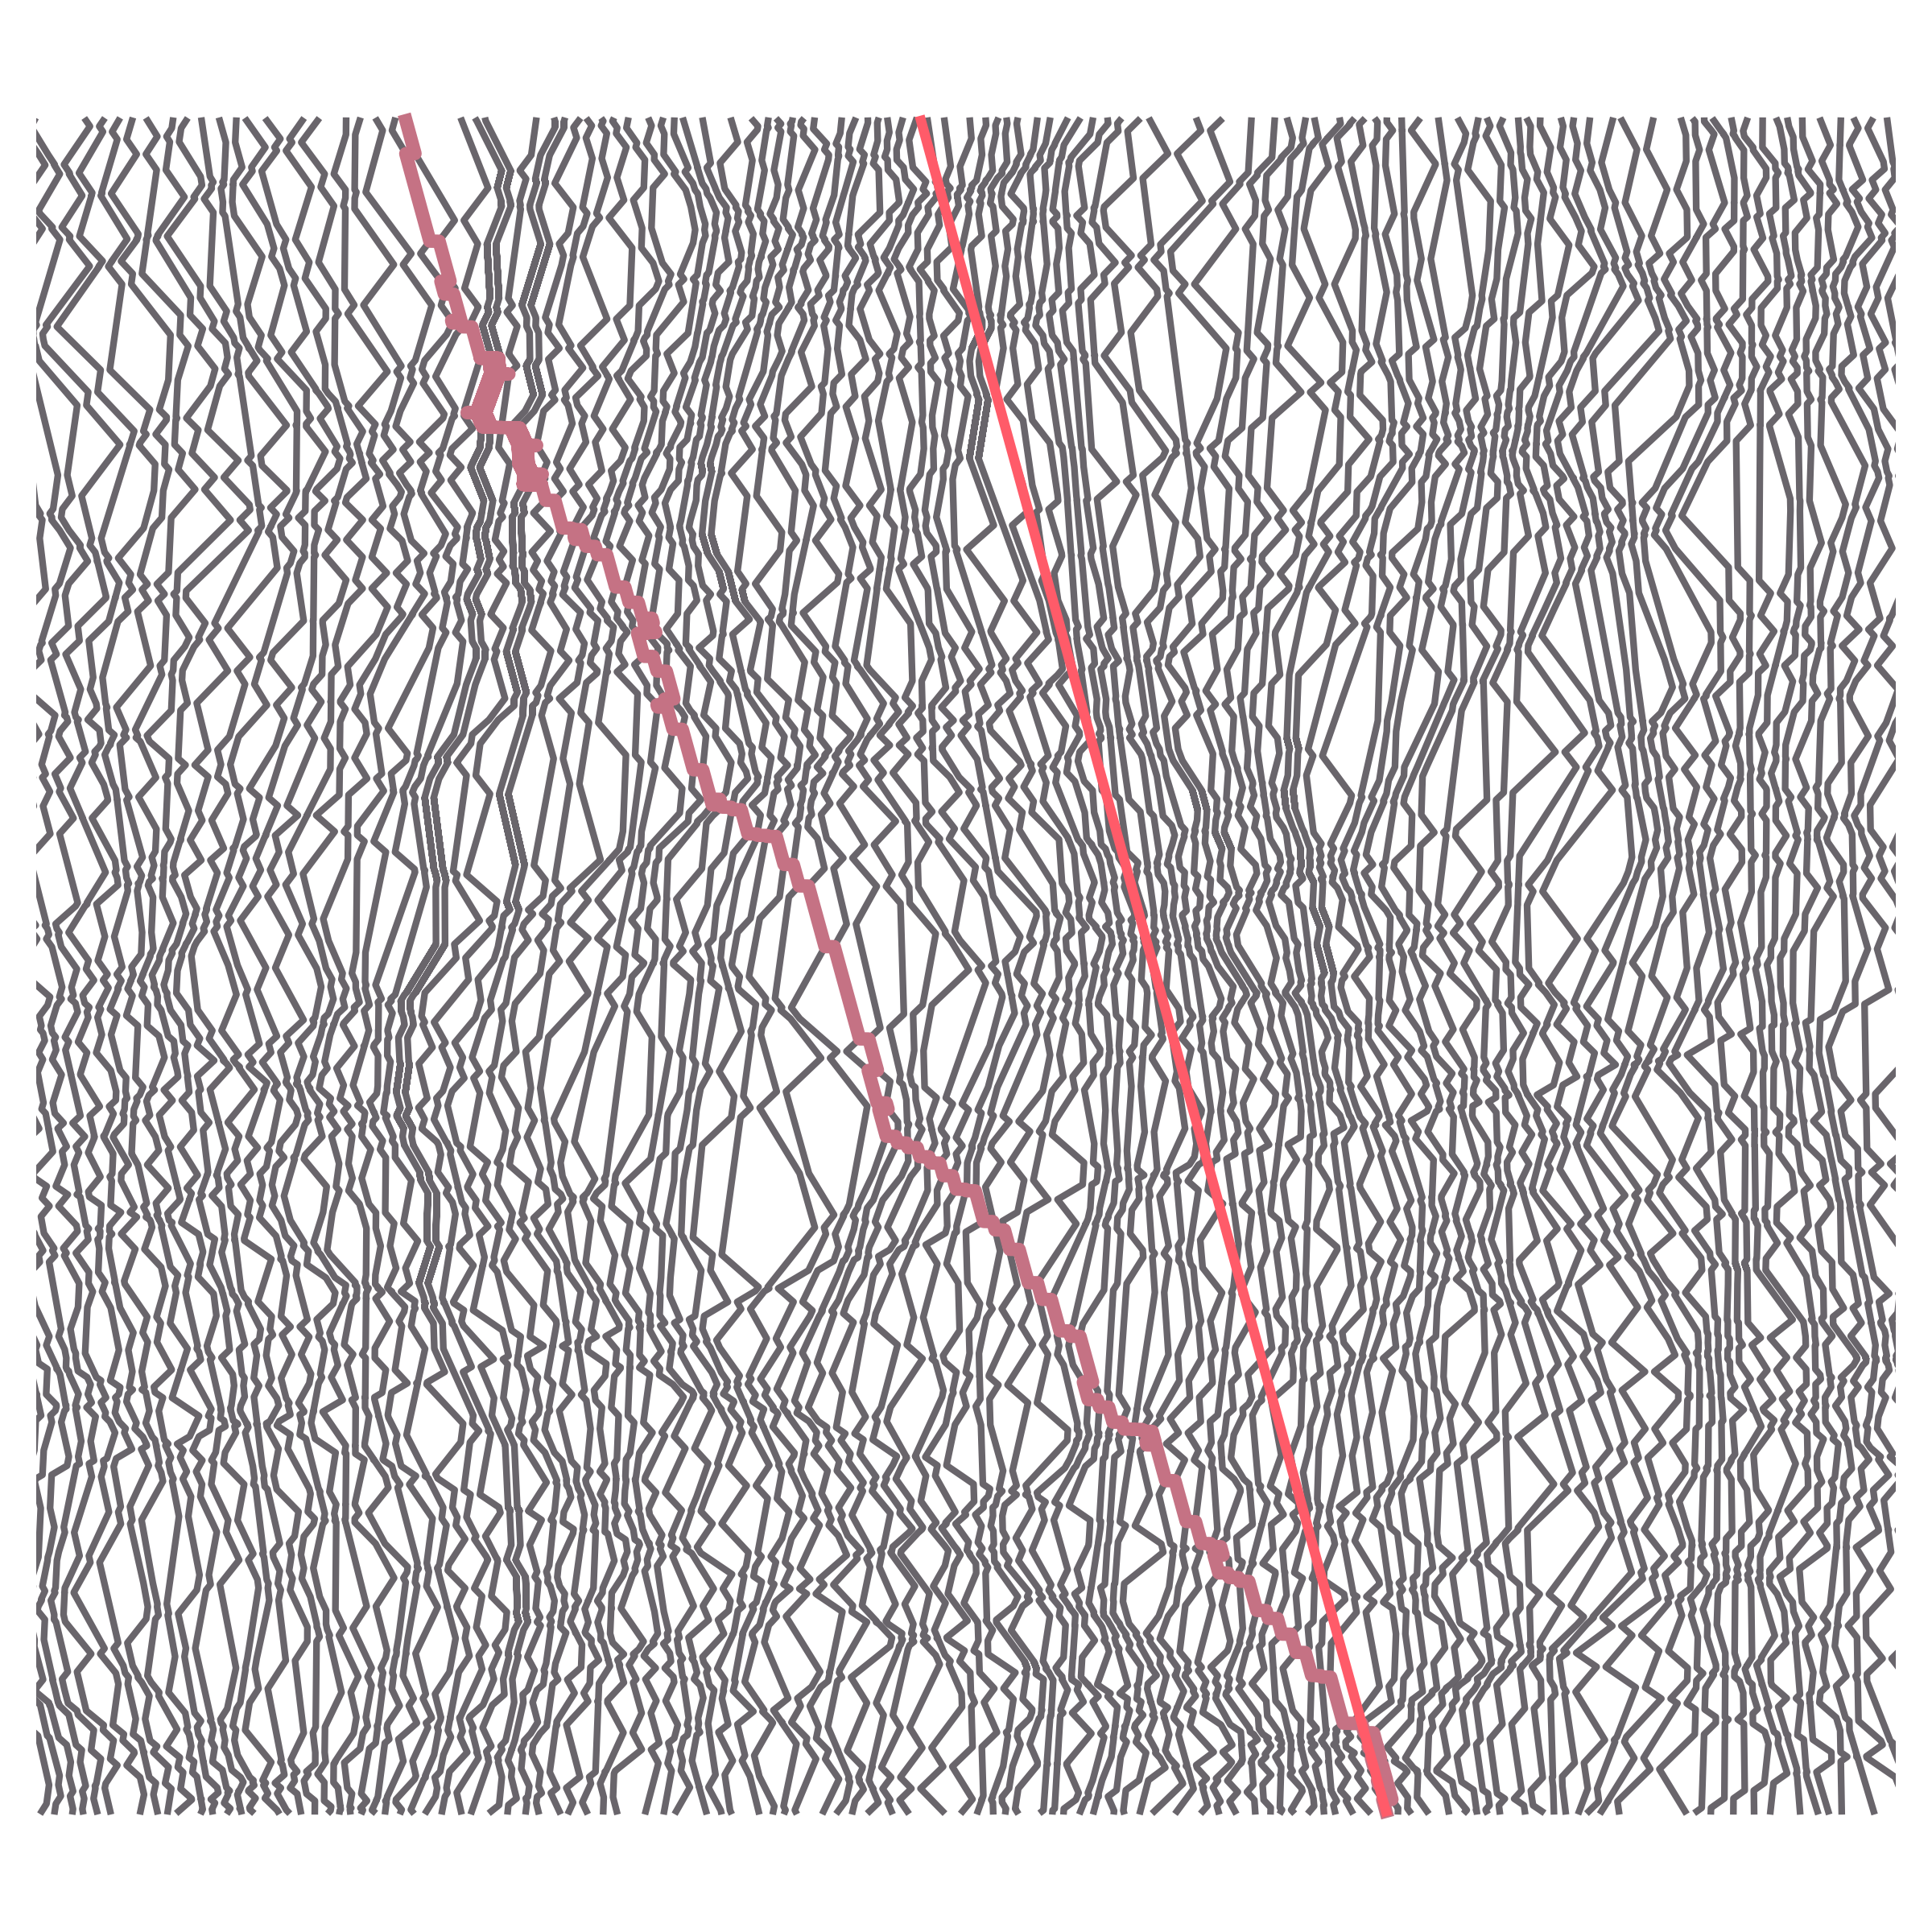
\includegraphics[width=0.8\textwidth]{figures/03_GHD/trajectoires_hard_rods.png}
    \caption{%Trajectoires des particules d'un gaz de hard rods en 1D. Les lignes noires représentent les particules individuelles, la ligne rouge correspond à la trajectoire effective (vitesse GHD) de la particule suivie, et la ligne orange indique la trajectoire de la particule si elle conservait sa vitesse initiale (bare velocity).
    Trajectoires des particules d'un gaz de barres dures en 1D. Les lignes noires représentent les particules individuelles, la ligne rouge la trajectoire effective (vitesse \gls{GHD}) de la particule suivie, et la ligne orange la trajectoire si la particule conservait sa vitesse initiale (bare velocity). Le graphique a été généré en Python.
    }
    \label{fig:trajectoires_hard_rods}
\end{figure}

\subsection{Diagonalisation et invariants de Riemann dans la GHD spatiale étendue}

%Nous nous restreignons au modèle de \gls{LL}.

%\medskip

En dérivant la définition de l'opération d’\emph{habillage} \eqref{eq:dressing}, on obtient la relation suivante :
\begin{equation}\label{chap:GHD:d.dressing.0}
	\partial_X \big( f^{\mathrm{dr}}_{[\nu]} \big) 
	= \partial_X f  +  \frac{\Delta}{2\pi} \star \big( \nu \, \partial_X f^{\mathrm{dr}}_{[\nu]} \big)  
	+ \frac{\Delta}{2\pi} \star \big( f^{\mathrm{dr}}_{[\nu]} \, \partial_X \nu \big), 	
\end{equation}
où les variables \(X \in \{  t, x, \theta \} \).  Soit 
% \begin{equation}\label{chap:GHD:d.dressing.0.0}
% 	\left ( 1 - \frac{\Delta}{2\pi} \star  \, \left ( \nu \, \times	 \, \right )  \right )  \partial_X \big( f^{\mathrm{dr}}_{[\nu]} \big) 
% 	= \partial_X f    
% 	+ \frac{\Delta}{2\pi} \star \big( f^{\mathrm{dr}}_{[\nu]} \, \partial_X \nu \big), 	
% \end{equation}
\begin{equation}\label{chap:GHD:d.dressing.0.0}
	\left(\mathrm{Id}-\widehat{K}_{\nu}\right) \partial_X \big( f^{\mathrm{dr}}_{[\nu]} \big) 
	= \partial_X f    
	+ \frac{\Delta}{2\pi} \star \big( f^{\mathrm{dr}}_{[\nu]} \, \partial_X \nu \big), 	
\end{equation}
% \left(\mathbb{1}-\widehat{K}_{[\nu]}\right)\partial_X f^{\mathrm{dr}}_{[\nu]},
% \left ( 1 - \frac{\Delta}{2\pi} \star  \left ( \nu \, \cdot	 \right )  \right )
où nous avons introduit l’opérateur linéaire \(\widehat{K}_{\nu}\) construit à partir de \(\big(\mathrm{Id}-\tfrac{\Delta}{2\pi}\star \nu \times \big)\) et de convolutions par \(\tfrac{\Delta}{2\pi}\) \ie 
\begin{equation}
	(\widehat{K}_{\nu} \,  g)(\theta) = \int d\theta'\, K_{\nu}(\theta,\theta') g(\theta'),\qquad K_{\nu}(\theta,\theta')=\frac{\Delta(\theta-\theta')}{2\pi}\,\nu(\theta').
\end{equation}



En utilisant la définition \eqref{eq:dressing}, on obtient également que 
\begin{equation}
	\big( \partial_X f \big)^{\mathrm{dr}}_{[\nu]} 
	= \left(\mathrm{Id}-\widehat{K}_{\nu}\right)^{-1} \partial_X f ,
\end{equation}
donc en injectant dans \eqref{chap:GHD:d.dressing.0.0} il vient que 
%\begin{equation}\label{chap:GHD:d.dressing.1}
%	\partial_X(f^{\mathrm{dr}}_{[\nu]}) = \left (\partial_X f \right )^{\mathrm{dr}}_{[\nu]} + \frac{\Delta}{2\pi} \star ( \nu (\partial_X f^{\mathrm{dr}}_{[\nu]}-\partial_X(f^{\mathrm{dr}}_{[\nu]})) )  +\frac{\Delta}{2\pi} \star ( f^{\mathrm{dr}}_{[\nu]} \partial_X \nu  ), 	
%\end{equation}
%
%comment ????
\begin{equation}\label{chap:GHD:d.dressing}
	\partial_X\!\left(f^{\mathrm{dr}}_{[\nu]}\right) 
	= \left(\partial_X f \right)^{\mathrm{dr}}_{[\nu]} 
	+ \widehat{\Theta} \!\left( f^{\mathrm{dr}}_{[\nu]} \,\partial_X \nu \right), 	
\end{equation}
% où \(X \in \{t, x, \theta\}\) et où nous avons introduit l’opérateur \(\Theta\) linéaire construit à partir de \(\left(\mathrm{Id}-\widehat{K}_{\nu}\right)^{-1}\) et de convolutions par \(\tfrac{\Delta}{2\pi}\) \ie
% \begin{equation}
% 	\Theta \equiv \left(Id-\widehat{K}_{\nu}\right)^{-1} 
% 	\, \frac{\Delta}{2\pi}\star
% \end{equation}

où \( X \in \{t, x, \theta\} \), et où nous avons introduit l’opérateur linéaire
\(\widehat{\Theta}\), défini comme la composition de l’inverse de l’opérateur
\(\mathrm{Id} - \widehat{K}_{\nu}\) avec la convolution par \(\tfrac{\Delta}{2\pi}\), \emph{i.e.}
\begin{equation}\label{eq:def_Theta}
    \widehat{\Theta}
    \;\doteq\;
    \left(\mathrm{Id} - \widehat{K}_{\nu}\right)^{-1}
    \circ
    \widehat{K}_{\mathrm{Id}},
\end{equation}
avec
\begin{equation}
	(\widehat{K}_{\mathrm{Id}} \,  g)(\theta) = \int d\theta'\, K_{\mathrm{Id}}(\theta,\theta') g(\theta'),\qquad K_{\mathrm{Id}}(\theta,\theta')=\frac{\Delta(\theta-\theta')}{2\pi}.
\end{equation}



\medskip
Les dérivations des équations \eqref{chap:GHD:eq.nu.v.a.1} donnent :
\begin{eqnarray}
	2\pi \partial_t \rho & = & 1^{\mathrm{dr}}_{[\nu]} \partial_t \nu + \nu \, \left (  ( \partial_t 1 )^{\mathrm{dr}}_{[\nu]}  + \widehat{\Theta} \left ( 1^{\mathrm{dr}}_{[\nu]} \partial_t \nu   \right ) \right )  \\
	2\pi \partial_x ( v^{\mathrm{eff}} \rho ) & = & (\partial_\theta h )^{\mathrm{dr}}_{[\nu]} \partial_x \nu + \nu \, \left (  ( \partial_x \partial_\theta h )^{\mathrm{dr}}_{[\nu]}  +  \widehat{\Theta} \left ( (\partial_\theta h)^{\mathrm{dr}}_{[\nu]} \partial_x \nu   \right ) \right )\\
	2\pi \partial_\theta ( a^{\mathrm{eff}} \rho ) & = & -(\partial_x h )^{\mathrm{dr}}_{[\nu]} \partial_\theta \nu - \nu \, \left (  ( \partial_\theta \partial_x h )^{\mathrm{dr}}_{[\nu]}  +  \widehat{\Theta} \left ( (\partial_x h)^{\mathrm{dr}}_{[\nu]} \partial_\theta \nu   \right ) \right )
\end{eqnarray}
%où \(\Theta\) est l'opérateur linéaire construit à partir de \(\big(1-\tfrac{\Delta}{2\pi}\star\nu\cdot\big)^{-1}\) et de convolutions par \(\tfrac{\Delta}{2\pi}\) (\ie $\(\Theta\) = \left ( 1 - \frac{\Delta}{2\pi} \star \nu \, \cdot	 \right )^{-1} \frac{\Delta}{2\pi} \star $ ) . 
En injectant  dans l'équation \gls{GHD} \eqref{chap:GHD:eq.GHD.1} on obtient après calculs (regroupement des termes et mise en facteur)  
%\begin{eqnarray}
%	\begin{array}{c}\left ( \left(\partial_t 1 \right)^{\mathrm{dr}} +  \left ( 1 + \left(\partial_x  \partial_\theta h  \right)^{\mathrm{dr}} - \left(\partial_\theta  \partial_x h  \right)^{\mathrm{dr}} \right ) \nu \, + \\ \left ( 1 + \left ( 1 -   \frac{\Delta}{2 \pi } \star \nu \cdot \right )^{-1} \frac{\Delta}{2 \pi } \star \right )   \left ( 1^{\mathrm{dr}} \partial_t v +  \left ( \partial_\theta h \right )^{\mathrm{dr}} \partial_x \nu -  \left ( \partial_x h \right )^{\mathrm{dr}} \partial_\theta \nu\right ) = 0  \end{array}. 
%\end{eqnarray}
\begin{eqnarray}
	\left ( \left(\partial_t 1 \right)^{\mathrm{dr}}  + \left(\partial_x  \partial_\theta h  \right)^{\mathrm{dr}} - \left(\partial_\theta  \partial_x h  \right)^{\mathrm{dr}} \right ) \nu \, + ( \mathrm{Id} + \widehat{\Theta} )    \left ( 1^{\mathrm{dr}} \partial_t v +  \left ( \partial_\theta h \right )^{\mathrm{dr}} \partial_x \nu -  \left ( \partial_x h \right )^{\mathrm{dr}} \partial_\theta \nu\right ) = 0  . 
\end{eqnarray}
Puisque \(\partial_t1=0\) et \(\partial_x\partial_\theta h=\partial_\theta\partial_x h\), le premier crochet s'annule. Il reste donc
\[
\Big(\mathrm{Id} + \widehat{\Theta} \Big)\Big( 1^{\mathrm{dr}}_{[\nu]}\,\partial_t\nu
+ (\partial_\theta h)^{\mathrm{dr}}_{[\nu]}\,\partial_x\nu
- (\partial_x h)^{\mathrm{dr}}_{[\nu]}\,\partial_\theta\nu \Big) = 0.
\]

Sous l'hypothèse standard d'inversibilité des opérateurs d'\emph{habillage} \Big (\ie\ \(\left(\mathrm{Id} - \widehat{K}_{\nu}\right)\)~ est inversible et \(\widehat{\Theta}\) n'a pas de noyau pathologique 
\footnote{
L'inversibilité de l'opérateur \(\left(\mathrm{Id} - \widehat{K}_{\nu}\right)\) est une condition technique garantissant que le système d'équations intégrales définissant l'opération de dressing possède une solution unique. En pratique, cela signifie que le noyau de convolution \(\tfrac{\Delta}{2\pi}\star\nu\) n'a pas de valeur propre égale à 1, ce qui assurerait une accumulation d'effets d'interaction menant à une singularité. Cette condition est généralement satisfaite pour les systèmes intégrables physiques dans les régimes d'intérêt (faibles densités, ou régimes thermodynamiquement stables). L'absence de noyau pathologique pour \(\widehat{\Theta}\) signifie quant à elle que cet opérateur ne possède pas de zéro du déterminant de Fredholm, assurant son caractère bien défini et injectif. Ces hypothèses standard permettent d'annuler le terme entre crochets dans l'équation précédente, conduisant ainsi à l'équation de transport \eqref{chap:GHD:eq.nu.1}.
} 
\Big ), on en déduit l'annulation du membre intérieur. En divisant par \(1^{\mathrm{dr}}_{[\nu]}\) on obtient l'équation de transport locale :
\begin{equation}\label{chap:GHD:eq.nu.1}
	\partial_t\nu + v^{\mathrm{eff}}\partial_x\nu + a^{\mathrm{eff}}\partial_\theta\nu = 0,
\end{equation}
(avec \(v^{\mathrm{eff}}=(\partial_\theta h)^{\mathrm{dr}}_{[\nu]}/1^{\mathrm{dr}}_{[\nu]}\) et \(a^{\mathrm{eff}}=-(\partial_x h)^{\mathrm{dr}}_{[\nu]}/1^{\mathrm{dr}}_{[\nu]}\)).  
  

\medskip

Dans les systèmes hyperboliques\footnote{
Un \emph{système hyperbolique} est un système d'équations aux dérivées partielles de la forme
\[
\partial_t \mathbf{u} + \mathbf{A}(x,t,\mathbf{u}) \cdot \partial_x \mathbf{u} = \mathbf{S}(x,t,\mathbf{u}),
\]
où $\mathbf{u}$ est un vecteur d'inconnues (ici les densités conservées ou les variables spectrales), $\mathbf{A}$ est une matrice (appelée matrice de flux ou jacobienne), et $\mathbf{S}$ représente les termes sources éventuels. Le système est dit \emph{hyperbolique} si la matrice $\mathbf{A}$ possède $N$ valeurs propres réelles distinctes (ou, plus généralement, réelles) et $N$ vecteurs propres linéairement indépendants. Cette structure assure que les perturbations se propagent à des vitesses finies et bien définies (les vitesses caractéristiques), ce qui permet une description dynamique stable et l'existence de solutions de type ondes. L'équation \gls{GHD}, avec ses vitesses effectives $v^{\mathrm{eff}}$ et $a^{\mathrm{eff}}$, possède cette structure hyperbolique, permettant ainsi une diagonalisation et l'identification des invariants de Riemann.
}, la \emph{diagonalisation} d'une équation consiste à trouver une transformation des variables qui permet de décomposer le système couplé en un ensemble de modes indépendants, appelés \emph{invariants de Riemann} ou \emph{modes normaux}. 


\medskip

Dans le cadre de la théorie \gls{GHD} spatiale étendue, l'équation d'évolution de la densité \(\rho(x,\theta,t)\) est couplée de manière non triviale en \((x,\theta)\) par la vitesse effective \(v^{\mathrm{eff}}\) et l'accélération effective \(a^{\mathrm{eff}}\). \footnote{Par « couplée de manière non triviale en $(x,\theta)$ » on entend que $\rho(x,\theta,t)$ ne se factorise pas en une dépendance séparée en $x$ et en $\theta$ : la valeur pour une rapidité donnée $\theta$ dépend des valeurs pour d'autres rapidités $\theta'$ (et parfois d'autres positions $x'$) via des opérateurs non locaux. Concrètement, le \emph{dressing} est un opérateur intégral qui couple toutes les composantes en $\theta$, par exemple
$$f^{\mathrm{dr}}(\theta)=f(\theta)+\int d\alpha\,T(\theta,\alpha)\,\nu(\alpha)\,f^{\mathrm{dr}}(\alpha),$$
ce qui signifie que $v^{\mathrm{eff}}$ et $a^{\mathrm{eff}}$ (qui sont construits à partir de quantités « dressed ») rendent l'évolution en $x$ pour une $\theta$ donnée dépendante de la distribution sur toutes les $\theta'$. Un « couplage trivial » serait, en revanche, une dépendance séparable ou purement locale (p.ex. $g(x)h(\theta)$).} 
La fonction d'occupation \(\nu(x,\theta ; t)\) est définie par une transformation non locale dite \emph{dressing} qui incorpore les interactions du système.




\medskip

Grâce à cela, on peut affirmer que la fonction $\nu (x , \theta)$  s’interprète comme un continuum d’{\bf invariants de Riemann}, c’est-à-dire des variables normales qui restent constantes le long des caractéristiques du système.\footnote{Par « restent constantes le long des caractéristiques du système », on entend que la valeur de $\nu(x,\theta;t)$ demeure inchangée lorsqu'on suit une particule (ou plus précisément une quasi-particule) le long de sa trajectoire dans l'espace $(x,\theta)$. Mathématiquement, cela s'exprime par $\frac{d\nu}{dt}\big|_{\text{caractéristique}} = 0$, où la dérivée est prise en suivant le mouvement selon les équations de transport \eqref{chap:GHD:eq.nu.1}. Autrement dit, même si $\nu(x,\theta;t)$ varie en fonction du temps et de la position lorsqu'on les observe en points fixes, elle reste constante le long des courbes caractéristiques définies par $\dot{x} = v^{\mathrm{eff}}(\theta)$ et $\dot{\theta} = a^{\mathrm{eff}}(x)$. C'est cette propriété qui fait de $\nu$ un véritable invariant de Riemann : chaque niveau de $\nu$ se propage selon ses propres caractéristiques sans se mélanger avec les autres niveaux, ce qui permet de diagonaliser entièrement la dynamique du système.}
En effet, l'équation de transport locale \eqref{chap:GHD:eq.nu.1} montre que \(\nu\) est conservée le long des trajectoires définies par les vitesses effectives \(v^{\mathrm{eff}}\) et les accélérations effectives \(a^{\mathrm{eff}}\). Autrement dit, chaque valeur de \(\nu\) pour une rapidité donnée \(\theta\) évolue indépendamment des autres, ce qui permet de diagonaliser le système d'équations couplées en un ensemble de modes indépendants.


\medskip

Cette diagonalisation \eqref{chap:GHD:eq.nu.1} est essentielle pour comprendre la structure hamiltonienne du système et simplifier l'analyse de sa dynamique, notamment dans le cadre spatialement étendu avec un dressing dépendant de la position. 
\footnote{
Par « diagonalisation », on entend le processus de transformation du système d'équations couplées \eqref{chap:GHD:eq.GHD.1} en un ensemble de modes découplés et indépendants. Dans le formalisme de la GHD, cela correspond à l'identification de la fonction d'occupation $\nu(x,\theta;t)$ comme un continuum d'invariants de Riemann. 

Mathématiquement, la diagonalisation s'exprime par le fait que l'équation de transport \eqref{chap:GHD:eq.nu.1}
\[
\partial_t\nu + v^{\mathrm{eff}}\partial_x\nu + a^{\mathrm{eff}}\partial_\theta\nu = 0
\]
peut être écrite sous la forme
\[
\frac{d\nu}{dt}\bigg|_{\text{car}} = 0,
\]
où la dérivée est prise le long des caractéristiques définies par $\dot{x} = v^{\mathrm{eff}}(\theta)$ et $\dot{\theta} = a^{\mathrm{eff}}(x)$. Cela signifie que chaque « niveau » de $\nu$ (chaque valeur de la fonction d'occupation pour une rapidité donnée) reste constant le long de sa trajectoire caractéristique dans l'espace $(x,\theta)$, sans se mélanger avec les autres niveaux. 

Cette propriété permet de résoudre le système complet non pas en tant que système couplé global, mais plutôt en suivant indépendamment l'évolution de chaque mode, ce qui simplifie drastiquement l'analyse dynamique même lorsque le dressing dépend explicitement de la position.
}

\section{Formulation hamiltonienne de la théorie Hydrodynamique Généralisée}

Dans  \cite{bonnemain2024hamiltonian}, il est montré que les équations \gls{GHD} peuvent
avoir une formulation Hamiltonienne dans le cadre d'une théorie de champ classique,
moyennant une redéfinition du crochet de Poisson. J'ai trouvé cette approche intéressante
et je présente ici ce résultat. En aucun cas les calculs ci-dessous ne sont une dérivation de \gls{GHD}.


\subsection{Crochet de Poisson fonctionnel}

% \paragraph{Interprétation et limite non-interactive}  
% À ce niveau de généralité, l'équation \gls{GHD} \eqref{chap:GHD:eq.GHD.1} peut être interprétée comme la dynamique hydrodynamique d’un fluide bidimensionnel dont la densité est conservée dans l’espace des phases spectral.  
% Les effets d’interaction se traduisent par un couplage non local dans la direction des rapidités $\theta$, reflétant les processus d'interactions entre quasi-particules possédant des paramètres spectraux distincts.

\paragraph{Interprétation et limite non-interactive}  
À ce niveau de généralité, l'équation \gls{GHD} \eqref{chap:GHD:eq.GHD.1} peut être interprétée comme la dynamique hydrodynamique d'un fluide bidimensionnel\footnote{Le terme « bidimensionnel » désigne ici l'espace des phases spectral $(x,\theta)$, et non l'espace physique. Les deux dimensions correspondent à : (i) la variable spatiale $x$ décrivant l'inhomogénéité du système dans l'espace physique réel, et (ii) la variable spectrale $\theta$ (la rapidité) caractérisant l'état asymptotique de chaque quasi-particule. La « densité » dans cet espace $(x,\theta)$ est précisément $\rho(x,\theta,t)$, la distribution locale de rapidité.} dont la densité est conservée dans l'espace des phases spectral.  
Les effets d'interaction se traduisent par un couplage non local dans la direction des rapidités $\theta$\footnote{Le « couplage non local en $\theta$ » signifie que l'évolution de $\rho(x,\theta,t)$ pour une rapidité donnée $\theta$ dépend non seulement de la distribution aux points voisins en $\theta$, mais aussi de la distribution sur l'ensemble du spectre de rapidités. Mathématiquement, cela se manifeste par des opérateurs intégraux, notamment le dressing $(\cdot)^{\mathrm{dr}}_{[\nu]}$ (équation \eqref{eq:dressing}), qui couple implicitement toutes les valeurs de $\theta'$ à travers des noyaux de convolution comme $\Delta(\theta-\theta')$ (voir équation \eqref{chap:GHD:veff.4}). Cette non-localité reflète le fait que, dans un système intégrable, les interactions à deux corps entre quasi-particules de rapidités différentes créent un couplage global : une quasi-particule à la rapidité $\theta$ « ressent » la présence de toutes les autres quasi-particules à d'autres rapidités $\theta'$, et sa dynamique en est affectée de façon non triviale.}, reflétant les processus d'interactions entre quasi-particules possédant des paramètres spectraux distincts\footnote{Par « paramètres spectraux distincts », on entend que deux quasi-particules ont des rapidités différentes, $\theta \neq \theta'$. Dans un système intégrable, les collisions binaires entre quasi-particules de rapidités différentes sont décrites par la matrice de diffusion (ou matrice $S$), caractérisée par la phase de diffusion $\varphi(\theta - \theta')$ ou le noyau de dressing $\Delta(\theta-\theta')$. Ces grandeurs dépendent de la différence relative des rapidités et encodent comment la présence d'une quasi-particule à rapidité $\theta'$ modifie le comportement effectif d'une quasi-particule à rapidité $\theta$. C'est précisément cette interaction sélective entre différents « modes » spectraux qui crée le couplage non local observable dans l'équation \gls{GHD}.}.

\medskip

Dans le cas limite d’un système \emph{sans interactions}, l’espace spectral coïncide avec l’espace des phases classiques, et l’équation \gls{GHD} se réduit alors à l’équation de Liouville (ou, de façon équivalente, à l’équation de Boltzmann sans terme de collisions) issue de la théorie cinétique élémentaire.

\medskip

En l’absence de phénomènes dissipatives, la densité de distribution $\rho$ est conservée le long du flot hamiltonien associé à l’énergie $H$, ce qui s’exprime par
\footnote{
	\textbf{Convention de signe pour l'équation de Liouville et le crochet de Poisson~:}
	Il existe deux conventions couramment utilisées dans la littérature. 
	La convention de \textbf{Dirac} (adoptée dans ce chapitre) définit l'équation de Liouville comme
	\[
	\frac{d\rho}{dt} = \frac{\partial\rho}{\partial t} + \{\rho, H\} = 0,
	\]
	où le crochet de Poisson canonique est $\{A,B\} = \sum_i \left(\frac{\partial A}{\partial q_i}\frac{\partial B}{\partial p_i} - \frac{\partial A}{\partial p_i}\frac{\partial B}{\partial q_i}\right)$.
	La convention de \textbf{Landau et Lifschitz} utilise une définition opposée du crochet, conduisant à $\frac{d\rho}{dt} = \frac{\partial\rho}{\partial t} - \{\rho, H\} = 0$.
	Ces deux formulations sont équivalentes mathématiquement, mais diffèrent par le signe du crochet de Poisson. 
	Dans ce manuscrit, nous suivons la convention de \textbf{Dirac}.
}
\begin{equation}\label{chap:GHD:eq.Liouv.1}
	\frac{d \rho}{dt} 
	= \frac{\partial \rho}{\partial t } + \{ \rho , H \} = 0,
\end{equation}
où $\{\bullet, \bullet\}$ désigne le crochet de Poisson canonique dans l’espace des phases.  
Dans cette perspective, la théorie \gls{GHD} apparaît comme une extension naturelle de l’équation de Liouville aux systèmes intégrables, incorporant les effets collectifs induits par les interactions tout en préservant une description exacte à grande échelle.\footnote{La théorie \gls{GHD} fournit, pour les modèles intégrables, une description rigoureuse de la dynamique à l'échelle d'Euler. Elle n'est pas une approximation de type champ moyen : elle résulte de la prise en compte explicite de l'infinité de lois de conservation caractéristiques de l'intégrabilité et, de ce fait, préserve la structure des corrélations et l'ensemble des charges conservées. Elle établit un lien cohérent entre la dynamique microscopique — l'évolution des quasi‑particules en variables spectrales \(\theta\) et spatiales \(x\) — et la dynamique macroscopique des densités résolues en rapidité, sans recours à des termes phénoménologiques intermédiaires. Enfin, dans la limite sans interactions l'espace spectral coïncide avec l'espace des phases classique et l'équation \gls{GHD} se réduit à l'équation de Liouville (équivalente à la formulation cinétique collisionless, p.ex. Vlasov/Boltzmann sans terme de collision).}


\paragraph{Structure hamiltonienne et crochet de Poisson fonctionnel}  
Bonnemain \emph{et al.} \cite{bonnemain2024hamiltonian} introduisent un crochet de Poisson fonctionnel agissant sur des fonctionnelles $F$ et $G$ de la distribution de rapidité $\rho(x,\theta)$ en présence d’interactions. Celui-ci s’écrit
\begin{equation}\label{chap:GHD:eq.chochet.bonnemain.1}
	\{F,G\}
	=\iint dx\,d\theta\;\frac{\nu}{2\pi}\,
	\left[
		\partial_x \left( \frac{\delta F}{\delta \rho(x,\theta)} \right)
		\left( \partial_\theta \left( \frac{\delta G}{\delta \rho(x,\theta)} \right) \right)^{\mathrm{dr}}_{[\nu]}
		-
		\partial_x \left( \frac{\delta G}{\delta \rho(x,\theta)} \right)
		\left( \partial_\theta \left( \frac{\delta F}{\delta \rho(x,\theta)} \right) \right)^{\mathrm{dr}}_{[\nu]}
	\right],
\end{equation}
où $\nu$ désigne la fonction d’occupation. Dans ce crochet l'application de l’opération d’\emph{habillage} $(\bullet)^{\mathrm{dr}}_{[\nu]}$ \eqref{eq:dressing}  traduit les interactions entre particules.

%L’opérateur de \emph{dressing} $(\cdot)^{\mathrm{dr}}_{[\nu]}$ agit ici sur les dérivées fonctionnelles dans la variable spectrale $\theta$ ; il encode les effets des interactions à longue portée dans l’espace des rapidités. Cette structure hamiltonienne permet de reformuler la GHD comme une équation de type Liouville sur l’espace fonctionnel des distributions $\rho$, mais avec un crochet de Poisson modifié par le \emph{dressing}, traduisant la nature intégrable et non-locale des interactions.

\medskip


Le crochet de Poisson (défini en~\eqref{chap:GHD:eq.chochet.bonnemain.1}) entre deux charges $\mathcal{Q}[f]$ et $\mathcal{Q}[g]$ prend la forme
\begin{equation}\label{chap:GHD:eq.chochet.bonnemain.2}
	\{\mathcal{Q}[f], \mathcal{Q}[g]\}
	= \int_{\mathbb{R}^2} dx\, d\theta\, \frac{\nu}{2\pi} 
	\left[ \partial_x f \, (\partial_\theta g)^{\mathrm{dr}}_{[\nu]} 
	     - \partial_x g \, (\partial_\theta f)^{\mathrm{dr}}_{[\nu]} \right].
\end{equation}
%où $\nu$ est la fonction d’occupation et $(\cdot)^{\mathrm{dr}}_{[\nu]}$ désigne l’application de \emph{dressing} associée à $\nu$.

\medskip

Cette application de \emph{dressing} satisfait la relation de symétrie~\cite{doyon2020lecture} :
\begin{equation}\label{chap:GHD:eq.sym.dr.1}
	\int_{\mathbb{R}^2} dx\, d\theta \; \nu \, f \, g^{\mathrm{dr}}_{[\nu]} 
	= \int_{\mathbb{R}^2} dx\, d\theta \; \nu \, f^{\mathrm{dr}}_{[\nu]} \, g.
\end{equation}

%Pour appliquer la relation de symétrie~\eqref{chap:GHD:eq.sym.dr.1} au crochet~\eqref{chap:GHD:eq.chochet.bonnemain.2}, il est nécessaire de vérifier que les fonctions impliquées satisfont les conditions requises sur leurs types tensoriels.
%\footnote{
%La relation de symétrie~\eqref{chap:GHD:eq.sym.dr.1} est valable lorsque la somme des types tensoriels de $f$ et $g$ est $(1,1)$ dans le sens de~\cite{doyon2020lecture}. Dans ce formalisme, le type $(a,b)$ caractérise la transformation d'un objet vis-à-vis de $x$ (première entrée) et de $\theta$ (seconde entrée). Si $f$ est de type $(p,q)$ et $g$ de type $(r,s)$, alors leur somme est $(p+r,q+s)$. La condition $(1,1)$ garantit que l'intégrande $\nu\, f\, g^{\mathrm{dr}}$ est un scalaire invariant, rendant l'intégrale bien définie. Dans~\eqref{chap:GHD:eq.chochet.bonnemain.2}, $\partial_x f$ est de type $(1,0)$ et $\partial_\theta g$ de type $(0,1)$, ce qui satisfait cette condition et permet l'utilisation de~\eqref{chap:GHD:eq.sym.dr.1}.
%}

Pour appliquer la relation de symétrie~\eqref{chap:GHD:eq.sym.dr.1} au crochet~\eqref{chap:GHD:eq.chochet.bonnemain.2}, il suffit de considérer que les fonctions impliquées $f$ et $g$ sont des fonctions scalaires régulières sur $(x,\theta)$. Dans ce cas, la relation de symétrie reste pleinement valide et l'intégrale est bien définie.

\footnote{La relation de symétrie~\eqref{chap:GHD:eq.sym.dr.1} stipule que 
\begin{equation*}
\int_{\mathbb{R}^2} dx\, d\theta \; \nu \, f \, g^{\mathrm{dr}}_{[\nu]} 
= \int_{\mathbb{R}^2} dx\, d\theta \; \nu \, f^{\mathrm{dr}}_{[\nu]} \, g,
\end{equation*}
ce qui signifie que l'intégrale double sur l'espace $(x,\theta)$ du membre de gauche égale celle du membre de droit. Cette symétrie de l'opérateur de dressing permet d'échanger l'action du dressing entre $g$ et $f$ à travers l'intégration, ce qui est crucial pour réduire le crochet~\eqref{chap:GHD:eq.chochet.bonnemain.2} à la forme compacte~\eqref{chap:GHD:eq.chochet.bonnemain.3}. Le formalisme des types tensoriels introduit dans~\cite{doyon2020lecture} sert à traiter des objets plus complexes (tenseurs dépendant de $x$ et $\theta$); pour des fonctions scalaires comme ici, aucune condition supplémentaire n'est nécessaire.}

En utilisant cette symétrie ainsi qu’une intégration par parties, le crochet~\eqref{chap:GHD:eq.chochet.bonnemain.2} se réécrit
\begin{equation}\label{chap:GHD:eq.chochet.bonnemain.3}
	\{\mathcal{Q}[f], \mathcal{Q}[g]\}
	= \int_{\mathbb{R}^2} dx\, d\theta \; f \,
	\left[
		\partial_\theta \left( \frac{\nu}{2\pi} \, (\partial_x g)^{\mathrm{dr}}_{[\nu]} \right)
		- \partial_x \left( \frac{\nu}{2\pi} \, (\partial_\theta g)^{\mathrm{dr}}_{[\nu]} \right)
	\right].
\end{equation}

\medskip

\subsection{Crochet avec l’Hamiltonien}

On reprend un Hamiltonien de la forme de \eqref{chap:GHD:eq.ham.1},  $H = \mathcal{Q}[h]$. 

\paragraph{Densité hamiltonienne et grandeurs effectives} 
%On note $h(x,\theta)$ la densité associée à la moyenne de l’Hamiltonien, telle que
%\begin{equation}\label{chap:GHD:eq.ham.1}
%	H = \mathcal{Q}[h].
%\end{equation}

%La fonction d’occupation $\nu$, la vitesse effective $v^{\mathrm{eff}}$ et l’accélération effective $a^{\mathrm{eff}}$ sont définies par
%\begin{equation}\label{chap:GHD:eq.nu.v.a.1}
%	\nu = 2\pi \frac{\rho}{1^{\mathrm{dr}}_{[\nu]}}, 
%	\quad v^{\mathrm{eff}} = \frac{(\partial_\theta h )^{\mathrm{dr}}_{[\nu]}}{1^{\mathrm{dr}}_{[\nu]}}, 
%	\quad a^{\mathrm{eff}} = -\frac{(\partial_x h )^{\mathrm{dr}}_{[\nu]}}{1^{\mathrm{dr}}_{[\nu]}},
%\end{equation}
%\begin{equation}\label{chap:GHD:eq.nu.v.a.1}
%	2 \pi \rho =  1^{\mathrm{dr}}_{[\nu]} \, \nu , 
%	\quad 2 \pi \, v^{\mathrm{eff}} \, \rho  =(\partial_\theta h )^{\mathrm{dr}}_{[\nu]} \, \nu , 
%	\quad 2 \pi \, a^{\mathrm{eff}} \, \rho  = -(\partial_x h )^{\mathrm{dr}}_{[\nu]}\, \nu ,
%\end{equation}
%toutes trois étant des fonctions de $\rho(\cdot,\cdot,t)$. 

% La vitesse effective et l'accélération effective données à l'équation \eqref{chap:GHD:eq.nu.v.a.1} interviennent dans les équations de mouvement
% \begin{equation}\label{chap:GHD:eq.nu.v.a.1.1}
% 	\dot{x} = v^{\mathrm{eff}}, \qquad \dot{\theta} = a^{\mathrm{eff}},
% \end{equation}
% montrant que les dérivées $\partial_x$ et $\partial_\theta$ présentes dans le crochet de Poisson correspondent respectivement à l'action de l'accélération effective sur $\theta$ et de la vitesse effective sur $x$.

\medskip

La vitesse effective et l'accélération effective données à l'équation \eqref{chap:GHD:eq.nu.v.a.1} interviennent dans les équations de mouvement\footnote{Ces équations de mouvement découlent de la structure hamiltonienne du système. Elles expriment que les variables conjuguées $x$ et $\theta$ évoluent selon les vitesses et accélérations effectives, qui encodent la dynamique complète du système dans le référentiel considéré.}
\begin{equation}\label{chap:GHD:eq.nu.v.a.1.1}
    \dot{x} = v^{\mathrm{eff}}, \qquad \dot{\theta} = a^{\mathrm{eff}},
\end{equation}
montrant que les dérivées $\partial_x$ et $\partial_\theta$ présentes dans le crochet de Poisson %$\{A, B\} = \partial_x A \partial_\theta B - \partial_\theta A \partial_x B$ 
correspondent respectivement aux générateurs infinitésimaux de l'évolution temporelle. Plus précisément :
\begin{itemize}[label = $\bullet$ ]
    \item $\partial_x$ agit comme le générateur des translations en $\theta$ via l'accélération effective $a^{\mathrm{eff}}$ ;
    \item $\partial_\theta$ agit comme le générateur des translations en $x$ via la vitesse effective $v^{\mathrm{eff}}$.
\end{itemize}
Ainsi, le crochet de Poisson encode le couplage entre ces deux degrés de liberté à travers les termes effectifs.

\medskip 

%Avec ces définitions, le crochet~\eqref{chap:GHD:eq.chochet.bonnemain.3} s’écrit
En utilisant la définition de $v^{\mathrm{eff}}$ et $a^{\mathrm{eff}}$ données à l'équation \eqref{chap:GHD:eq.nu.v.a.1}, on trouve que le crochet \eqref{chap:GHD:eq.chochet.bonnemain.3} appliqué à $(f,h)$ devient 
\begin{equation}\label{chap:GHD:eq.chochet.bonnemain.4}
	\{\mathcal{Q}[f], \mathcal{Q}[h]\} 
	= - \int_{\mathbb{R}^2} dx\, d\theta \; f \left[ \partial_x \big( \rho \, v^{\mathrm{eff}} \big) 
	+ \partial_\theta \big( \rho \, a^{\mathrm{eff}} \big) \right].
\end{equation}

\paragraph{Forme locale : densités conservées .} 
En choisissant $(x,\theta) \mapsto \delta(\cdot - x)f(\theta)$ dans \eqref{chap:GHD:eq.charge.global.1}, on obtient la moyenne de la densité conservée \ie
%On remarque que les moyennes des densités conservées $q_{[f]}(x)$ s’obtiennent en appliquant la prescription
%\[
%(x,\theta) \mapsto \delta(\cdot - x) \, f(\theta)
%\]
%dans~\eqref{chap:GHD:eq.charge.global.1}, \emph{i.e.}
\begin{equation}\label{chap:GHD:eq.chochet.bonnemain.4.11}
	q_{[f]}(x,t) = \mathcal{Q} \big[ (x,\theta) \mapsto \delta(\cdot - x) \, f(\theta) \big] =\int d\theta\, f(\theta)\,\rho(x,\theta,t).
\end{equation}

Appliqué à~\eqref{chap:GHD:eq.chochet.bonnemain.4}, on obtient
\begin{equation}\label{chap:GHD:eq.chochet.bonnemain.5}
	\{q_{[f]}(x), \mathcal{Q}[h]\} 
	= - \partial_x \left[ \int_{\mathbb{R}} d\theta \; f \, \rho \, v^{\mathrm{eff}} \right]
	+ \int_{\mathbb{R}} d\theta \; f' \, \rho \, a^{\mathrm{eff}}.
\end{equation}

En appliquant l’équation de Liouville~\eqref{chap:GHD:eq.Liouv.1} , on retrouve la forme de convection~\eqref{chap:GHD:eq.conserv.1} :
\begin{equation}\label{chap:GHD:eq.conserv.2}
	\partial_t q_{[f]} + \partial_x j_{[f]} = F_{[f]},
\end{equation}
où le flux $j_{[f]}$ et le terme de force $F_{[f]}$ sont donnés par
\begin{equation}\label{chap:GHD:eq.conserv.2.1}
	j_{[f]} = \int_{\mathbb{R}} d\theta \; v^{\mathrm{eff}} \, f \, \rho,
	\quad F_{[f]} = \int_{\mathbb{R}} d\theta \; a^{\mathrm{eff}} \, f' \, \rho.
\end{equation}

\paragraph{Forme locale : équation sur \texorpdfstring{$\rho$}{rho}} 
De manière analogue, pour la distribution de rapidité à l’équilibre thermodynamique, on note
\begin{equation}
	\rho(x,\theta) = \mathcal{Q}\big[ \delta(\cdot - x) \, \delta(\cdot - \theta) \big].
\end{equation}
Appliqué à~\eqref{chap:GHD:eq.chochet.bonnemain.4}, on obtient
\begin{equation}\label{chap:GHD:eq.chochet.bonnemain.6}
	\{\rho(x,\theta), \mathcal{Q}[h]\} 
	= - \partial_x \big( v^{\mathrm{eff}} \, \rho \big)
	  - \partial_\theta \big( a^{\mathrm{eff}} \, \rho \big).
\end{equation}

% En appliquant l’équation de Liouville~\eqref{chap:GHD:eq.Liouv.1}, on retrouve l’équation \gls{GHD}~\eqref{chap:GHD:eq.GHD.1} :
% \begin{equation*}\label{chap:GHD:eq.conserv.3}
% 	\partial_t \rho + \partial_x \big( v^{\mathrm{eff}} \rho \big)
% 	+ \partial_\theta \big( a^{\mathrm{eff}} \rho \big) = 0.
% \end{equation*}

{\color{blue}
En appliquant l’équation de Liouville~\eqref{chap:GHD:eq.Liouv.1} ($\partial_t \rho(x,\theta,t) = \{\rho(x,\theta,t), H\}$), on retrouve l’équation \gls{GHD}~\eqref{chap:GHD:eq.GHD.1}%\footnote{Remarque sur la convention de signe~: nous utilisons ici la convention \(\dfrac{d\rho}{dt}=\partial_t\rho+\{\rho,H\}=0\) (voir \eqref{chap:GHD:eq.Liouv.1}); avec le crochet de Poisson défini en \eqref{chap:GHD:eq.chochet.bonnemain.1} cela conduit précisément au signe présent dans \eqref{chap:GHD:eq.chochet.bonnemain.6}, il n'y a donc pas d'erreur de signe.} 
:
\begin{equation*}\label{chap:GHD:eq.conserv.3}
	\partial_t \rho + \partial_x \big( v^{\mathrm{eff}} \rho \big)
	+ \partial_\theta \big( a^{\mathrm{eff}} \rho \big) = 0.
\end{equation*}

}




%\section{Cas particuliers et interpretations}
\subsection{Modèle de Lieb–Liniger}

%Les informations relatives aux interactions entre particules sont contenues dans la définition du crochet de Poisson \eqref{chap:GHD:eq.chochet.bonnemain.1}, associée à l’opérateur de \emph{dressing} spécifique au modèle de Lieb–Liniger, défini en \eqref{eq:dessing}.  
Dans le modèle de \gls{LL}, l’Hamiltonien $H = \mathcal{Q}[h]$ \eqref{chap:GHD:eq.ham.1} s’écrit ici avec :
\begin{equation}\label{chap:GHD:eq.ham.2}
	h(x , \theta ) = \varepsilon(\theta) + V(x),
\end{equation}
où l’énergie cinétique est $\varepsilon(\theta) = \theta^2 / 2$ et $V(x)$ représente le potentiel extérieur.

\medskip

Dans ce modèle, la vitesse effective et l’accélération effective de \eqref{chap:GHD:eq.nu.v.a.1} se réécrivent :
\begin{equation}\label{chap:GHD:eq.nu.v.a.1.1111}
	v^{\mathrm{eff}} = \frac{(\mathrm{Id})^{\mathrm{dr}}_{[\nu]}}{1^{\mathrm{dr}}_{[\nu]}}, 
	\quad a^{\mathrm{eff}} = - V'(x).
\end{equation}

Avec l'equation \eqref{chap:GHD:veff.4} la vitesse effectif dans le modèle de \gls{LL} vérifie : 
\begin{equation}
	v^{\mathrm{eff}} = \theta +	\int d \theta' \, \Delta(\theta - \theta') \rho ( \theta') ( v^{\mathrm{eff}} ( \theta' ) - v^{\mathrm{eff}} ( \theta )  ) 
\end{equation}


Ainsi, les termes de force dans \eqref{chap:GHD:eq.conserv.2} et \eqref{chap:GHD:eq.conserv.2.1} prennent la forme :
\begin{equation}
	F_{[f]} = -V'(x) \int_{\mathbb{R}} d\theta \, f'(\theta) \, \rho(x, \theta).
\end{equation}

L’équation GHD \eqref{chap:GHD:eq.GHD.1} devient alors :
\begin{equation}\label{chap:GHD:eq.conserv.3.1}
	\partial_t \rho + \partial_x\!\left(v^{\mathrm{eff}} \rho\right) - V'(x) \, \partial_\theta \rho = 0,
\end{equation}
et \eqref{chap:GHD:eq.nu.1} devient :
\begin{equation}\label{chap:GHD:eq.nu.1.1}
	\partial_t \nu + v^{\mathrm{eff}}\partial_x \nu - V'(x) \, \partial_\theta \rho = 0,
\end{equation}



%\subsection{Cas sans interaction}
%
%\paragraph{Hypothèse ``sans interactions'' : $^{\rm dr}=\mathrm{Id}$.}
%Si l’opérateur d’habillage est l’identité (\emph{no dressing}), les crochet \eqref{chap:GHD:eq.chochet.bonnemain.1} et \eqref{chap:GHD:eq.chochet.bonnemain.4} se simplifient en :

\subsection{Cas ``no dressing''}

\paragraph{Hypothèse ``opérateur d’habillage identité'' : $^{\rm dr}=\mathrm{Id}$.}  
Si l’opérateur d’habillage correspond à l’identité (\emph{no dressing}), les crochets \eqref{chap:GHD:eq.chochet.bonnemain.1} et \eqref{chap:GHD:eq.chochet.bonnemain.4} se simplifient en :
\begin{eqnarray}
	\{F,G\} & = &  \iint dx\,d\theta\;\rho \,\left[\partial_x \!\left( \frac{\delta F}{\delta \rho (x , \theta)} \right)\, \partial_\theta \!\left( \frac{\delta G}{\delta \rho (x , \theta)} \right) - \partial_x \!\left( \frac{\delta G}{\delta \rho (x , \theta)} \right) \, \partial_\theta \!\left( \frac{\delta F}{\delta \rho(x , \theta) } \right) \right],\\
	\{\mathcal{Q}[f], \mathcal{Q}[h]\} &=& - \int_{\mathbb{R}^2} dx\, d\theta \; f \left[ \partial_x \big( \rho \, v^{\mathrm{eff}} \big) 
	+ \partial_\theta \big( \rho \, a^{\mathrm{eff}} \big) \right].
\end{eqnarray}
Les flux et termes de force \eqref{chap:GHD:eq.conserv.2.1} s’expriment alors en remplaçant la vitesse effective $v^{\mathrm{eff}}$ et l’accélération effective $a^{\mathrm{eff}}$ (de \eqref{chap:GHD:eq.nu.v.a.1}) par leurs expressions issues de la dynamique hamiltonienne \emph{nue} :
\begin{equation}
	\nu = 2\pi \rho, \qquad v^{\rm eff}(\theta)\ \to\ \partial_\theta h(x,\theta), \qquad a^{\rm eff}(\theta)\ \to\ -\partial_x h(x,\theta),
\end{equation}
où $h(x,\theta)$ est l’hamiltonien \emph{nu} (par exemple $h=\varepsilon(\theta)+V(x)$). 
Dans la limite sans interactions, l’équation \eqref{chap:GHD:eq.GHD.1} se réduit à une équation de transport sans collisions (de type Vlasov) :
\footnote{L'équation de Vlasov décrit l'évolution d'une distribution de particules dans l'espace des phases, en tenant compte des interactions entre particules. Elle est souvent utilisée pour modéliser des systèmes de particules dans des contextes où les effets de collision peuvent être négligés, permettant ainsi d'étudier la dynamique des systèmes en équilibre ou quasi-équilibre.}
\begin{equation}\label{eq:transport-libre}
  \partial_t \rho + \partial_x\!\big( \partial_\theta h\ \rho \big)
  - \partial_\theta\!\big( \partial_x h\ \rho \big) = 0.
\end{equation}

\paragraph{Hiérarchie des moments (charges nues).}
Pour toute fonction test $f(\theta)$, l'équation \eqref{chap:GHD:eq.chochet.bonnemain.5} devient
\begin{eqnarray}\label{chap:GHD:eq.flux.1}
j_{[f]}(x,t)=\int d\theta\, f(\theta)\,\partial_\theta h\,\rho(x,\theta,t), \qquad F_{[f]}(x,t) = -\int_{\mathbb{R}} d\theta \; \partial_x h \, f'(\theta)  \, \rho(x,\theta,t).
\end{eqnarray}

Pour $f(\theta) = 1$, $\theta$ et $\theta^2/2$ et $h(\theta,x)=\varepsilon(\theta)+V(x)$, l'équation \eqref{chap:GHD:eq.conserv.2} avec la charge locale \eqref{chap:GHD:eq.chochet.bonnemain.4.11} et les flux et forces \eqref{chap:GHD:eq.flux.1}, déviennent les équations d’Euler classiques (Annexe \ref{annex:Euler}) :
\begin{eqnarray}\label{chap:3:eq:hydro.1}
	\left\{
	\begin{array}{rcl}
	\partial_t n + \partial_x (n u) &=& 0, \\
	\partial_t (n u) + \partial_x (nu^2 + \mathcal{P}) &=& -\, n\partial_x V(x), \\
	\partial_t E + \partial_x (u\,(E+\mathcal{P})\,) &=& 0,
	\end{array}
	\right .  
\end{eqnarray}
avec la densité de particule $n = q_{[1]}$, la vitesse moyenne du fluide $u = {q_{[\theta]}}/{q_{[1]}}$ , la pression cinétique du fluide $\mathcal{P} =  q_{[\theta^2]} - {q_{[\theta]}^2}/{q_{[1]}} $ , l'énergie totale $E = nu^2/2 + nV + ne_{\rm int}$ où $e_{\rm int} = q_{[\theta^2/2]}$ est l'énergie interne d'une particule .



\paragraph{Remarques sur les charges globales.}
En l’absence de potentiel externe ($V = 0$), le système conserve certaines charges globales.

\smallskip

On a vu que dans un système classique non intégrable, seules ces quelques charges sont conservées. Par exemple dans un système de \gls{GE} sont conservés , nombre total de particules , quantité de mouvement totale, énergie cinétique totale soit respectivement $\mathcal{Q}[1]  =  \int dx \, q_{[1]}$, $\mathcal{Q}[\theta] = \int dx \, q_{[\theta]}$ et $\mathcal{Q}[{\theta^2}/{2}] = \int dx \, q_{\left[{\theta^2}/{2}\right]} $. 


\medskip

Et on a vu qu'en revanche, dans un système intégrable, une infinité de charges est conservée $\mathcal{Q}[(x,\theta) \mapsto f(\theta)]  =  \int dx \, q_{[(x,\theta) \mapsto f(\theta)]}$. En particulier, dans l'espace $(x,\theta)$, les nombres de rapidité dans chaque intervalle $[\theta , \theta + d\theta]$ est conservé :
\begin{equation*}
\Pi(\theta) \delta \theta  = Q[(x,\theta)  \mapsto \delta(\cdot - \theta) \,  \delta \theta ] = \int dx \, \rho(x,\theta;t)\,  \delta \theta.
\end{equation*}
Cela exprime que les rapidités situées dans une tranche $[\theta , \theta + d\theta]$ se déplacent en restant dans cette tranche, sans interagir ni s’échanger avec les autres tranches de rapidités.

\smallskip

Pour chaque valeur de $\theta$, la quantité $\Pi(\theta) \delta \theta$ est une charge globale conservée. Et pour chaque valeur de $\theta$, $\Pi(\theta) \delta \theta$ respecte une équation de continuité locale de type \eqref{chap:GHD:eq.conserv.1} sans terme de force. On a donc une infinité d'équations de continuité. Quand $\delta \theta \to 0$, on retrouve l'équation \gls{GHD} \eqref{chap:GHD:eq.GHD.1} sans terme de force
\begin{equation}
	\partial_t \rho + \partial_x \!\left(v^{\text{eff}} \rho\right)  = 0.
\end{equation}

Un potentiel externe $V(x)$ non nul induit, dans l’espace $(x,\theta)$, un couplage entre les différentes tranches de rapidités : c’est-à-dire qu’il provoque un transport des rapidités selon $x$, reliant ainsi des tranches de rapidités.

\medskip

Cette structure constitue l’analogue classique de la description en termes de {\bf distribution de rapidité} dans le cadre intégrable et fournit le point de départ naturel pour comprendre la théorie \gls{GHD}. 

\medskip
 
En particulier, pour décrire la dynamique à l’échelle d’Euler, il devient nécessaire de suivre l’évolution de \(\rho(x,\theta,t)\) pour toutes les valeurs de \(\theta\), contrairement au cas non intégrable où seules quelques densités locales suffisent.





\section{Régime de quasi-condensation et limite Gross--Pitaevskii}


Dans cette section, nous considérons un système décrit par le modèle \gls*{LL} ,sans potentiel extérieur,  dans le régime (\gls{qBEC}), correspondant à la limite $\mathfrak{t} \to 0$ et $\gamma \to 0$ (paramètres (température réduite et paramètre de Lieb)  définis en \eqref{chap2:eq:t.1} et \eqref{chap2:eq:gamma.1}).  Dans ces conditions, la dynamique du gaz peut être décrite par les équations hydrodynamiques issues de l’équation de \acrfull{GP}. L’objectif est de montrer que les équations de \gls{GHD} reproduisent, dans certaines situations\footnote{
Par « dans certaines situations », on entend précisément le cas où le système initial correspond à une distribution de rapidité formant une unique mer de Fermi, c'est-à-dire une fonction d'occupation $\nu(x,\theta,t)$ qui prend la valeur 1 dans un intervalle $[\theta_-(x,t), \theta_+(x,t)]$ et 0 ailleurs. Cette restriction est importante car si le système initial contient plusieurs structures (par exemple deux ou plusieurs mers de Fermi distinctes), la correspondance avec les équations de Gross–Pitaevskii n'est plus valide, comme nous le discuterons ultérieurement (voir remarque page~\pageref{rem:plusieurs_mers}). La limite $\gamma \to 0$ garantit également que les interactions restent faibles et que l'approximation de Thomas–Fermi (négligeant la pression quantique) demeure justifiée.
}, les équations hydrodynamiques dérivées de \gls{GP}.




\subsection{Évolution temporelle selon l’équation de Gross--Pitaevskii}
 
Dans le régime \gls{qBEC}, la dynamique d’un gaz unidimensionnel décrit par le modèle \gls{LL} à l’état fondamental peut être décrite par l’équation \gls{GP} dépendante du temps.
On a vu l'équation \gls{GP} dépendante du temps dans \eqref{chap.1:eq.GP.2}, avec $\hbar = m = 1$. Pour généraliser et pour l'utiliser dans un autre chapitre (\ref{chap:disp.exp}), écrivons-la avec un potentiel externe :
\begin{eqnarray}\label{chap.2:eq.GP.2}
	i \partial_t \psi = \left( - \frac{1}{2} \partial_x^2 + V + g \vert \psi \vert^2 \right) \psi .
\end{eqnarray}

En utilisant la représentation de \emph{Madelung} $\psi(x,t) = \sqrt{n(x,t)}\, e^{i\theta(x,t)}$, on obtient les équations dites hydrodynamiques de la forme de \eqref{chap:3:eq:hydro.1} \cite{Spiegel1980FluidDF,10.1093/acprof:oso/9780198758884.001.0001} :  
\begin{eqnarray}
    \partial_t n + \partial_x \big( n u \big) &=& 0, \label{eq:continuite}\\
    \partial_t (n u) + \partial_x \left( n u^2 + \mathcal{P} + \tilde{\mathcal{P}}_Q \right) &=& - n \partial_x V , \label{eq:euler}
\end{eqnarray}
où la vitesse du fluide, la \emph{pression classique} et un terme de \emph{pression quantique} sont définis par
\footnote{
\textbf{Distinction entre pression classique et pression quantique~:}
La \emph{pression classique} $\mathcal{P} = \frac{1}{2}gn^2$ provient du terme d'interaction répulsive de contact dans l'hamiltonien de \gls{GP}. Elle représente l'effet des collisions répulsives entre particules, analogue à la pression d'un gaz classique due aux chocs entre molécules. Elle dépend uniquement de la densité locale $n$.

La \emph{pression quantique} $\tilde{\mathcal{P}}_Q = -\frac{n}{2}\partial_x\left(\frac{\partial_x\sqrt{n}}{\sqrt{n}}\right)$ est un effet purement quantique, absent en mécanique classique. Elle provient de l'énergie cinétique des gradients de densité et est directement liée au principe d'incertitude~: confiner des particules dans une région de densité élevée augmente leur quantité de mouvement (et donc leur énergie). Mathématiquement, ce terme émerge de la contribution $-\frac{1}{2}\partial_x^2\sqrt{n}$ de l'énergie cinétique dans la décomposition de \emph{Madelung}. Dans la limite \acrfull{TF} ($\gamma \to 0$), le gradient de densité varie lentement et ce terme devient négligeable devant la pression classique.
}
\begin{equation}\label{eq:vitesse}
    u = \partial_x \theta, \quad 
    \mathcal{P} = \frac{1}{2} g n^2 , \quad 
    \tilde{\mathcal{P}}_Q = - \frac{n}{2} \partial_x \left( \frac{\partial_x \sqrt{n}}{\sqrt{n}} \right) .
\end{equation}


On peut aussi écrire \eqref{eq:euler} sous la forme
\begin{eqnarray}
	\partial_t u + \partial_x \left( \frac{u^2}{2} + \frac{2 \mathcal{P} + \mathcal{P}_Q}{n} + V \right) &=& 0, \label{eq:euler2}	
\end{eqnarray}
où l'on nomme dans la littérature la \emph{pression quantique} :
\begin{eqnarray}
	\mathcal{P}_Q = \frac{1}{2} \sqrt{n} \, \partial_x^2 \sqrt{n}.
\end{eqnarray}

\medskip
%Nous continuons avec \eqref{eq:continuite} et \eqref{eq:euler} sans potentiel externe $V$.
Dans la suite nous nous intéressons à la dynamique en l'absence de potentiel exterieur $V$.
  

%\medskip
%Dans la limite dite de \gls{TF} 1D, les fluctuations de densité sont faibles et le terme de \emph{pression quantique} peut être négligé \cite{PhysRevA.58.2385}. On retrouve alors la relation d’état 
%\(
%   \mu = g n
%\)
%liée à l’équilibre statique du système.

\medskip
Dans la limite dite de \gls{TF} 1D, les fluctuations de densité sont faibles et le terme de \emph{pression quantique} peuvent être négligé \cite{PhysRevA.58.2385}.  Le terme de pression se réduit alors à la pression classique 
\(
    \mathcal{P} = \frac{1}{2} g n^2.
\)
En utilisant la relation de Gibbs-Duhem 
\(
    \frac{d\mathcal{P}}{d\mu} = n,
\)
on obtient l’équation d’état classique du gaz \gls{qBEC} : 
\begin{equation}
    \mu = g n + cts.
\end{equation}

Les équations de \emph{Madelung} (\eqref{eq:continuite} \eqref{eq:euler}), se réduisent à :
\begin{eqnarray}
    \partial_t n + \partial_x \big( n u \big) &=& 0, \label{eq:continuite3}\\
    \partial_t (n u) + \partial_x \left( n u^2 + \mathcal{P} \right) &=& 0 \label{eq:euler3}.
\end{eqnarray}

\subsection{Description par les équations Hydrodynamiques Généralisées} 
 
Dans la suite, nous allons montrer que les équations \eqref{eq:continuite3} et \eqref{eq:euler3} peuvent être retrouvées à partir des équations \gls{GHD}.

\medskip

À $\mathfrak{t}=0$, le facteur d’occupation $\nu(x,\theta,0)$ ne peut prendre que deux valeurs :  il vaut $1$ si $\theta$ appartient à l’intervalle $[\theta_-(x,0),\, \theta_+(x,0)]$, et $0$ sinon.  Comme $\nu$ satisfait l’équation de transport \eqref{chap:GHD:eq.nu.1.1}, sa valeur est conservée le long des caractéristiques. \\ 

Ainsi, la distribution prend la forme d’une \emph{mer de Fermi}, délimitée par deux bords $\theta_\pm(x,t)$ :  

\begin{equation}\label{eq:merFermi}
    \nu(x,\theta,t) = 
    \begin{cases}
        1, & \theta \in [\theta_-(x,t), \theta_+(x,t)], \\
        0, & \text{sinon}.
    \end{cases}
\end{equation}
L’évolution temporelle des bords est donnée par deux équations de type transport (Fig ~\ref{fig:GP}) \cite{PhysRevLett.119.195301}:  
\begin{eqnarray}
    \partial_t \theta_+(x,t) + v^{\mathrm{eff}}(\theta_+) \, \partial_x \theta_+(x,t) &=& 0, \label{eq:theta+}\\
    \partial_t \theta_-(x,t) + v^{\mathrm{eff}}(\theta_-) \, \partial_x \theta_-(x,t) &=& 0. \label{eq:theta-}
\end{eqnarray}

%\subparagraph{Vitesse efficace aux bords de la mer de Fermi.}  
%La vitesse du fluide au point $x$ n'est rien d'autre que 
%\begin{equation}
%	u = \frac{\theta_- + \theta_+}2.
%\end{equation}
%Dans la limite $\gamma \to 0$, la distribution de rapidité est de la forme d'un demi-cercle \cite{LL_1963_1}\( \rho (\theta) = \sqrt{-(\theta - \theta_-)(\theta - \theta_+)} n /(2\pi c^2) \) avec la vitesse du son 
%\begin{equation}
%	c=\sqrt{gn},	
%\end{equation}, la largeur de la mer de fermi ($\theta_+-\theta_-$ ) est reliée à la densité par la relation $n = \int d\theta \rho(\theta)$, donne  :
%\begin{equation}
%	1 =  \left ( \frac{\theta_+ - \theta_-}{4 c}  \right )^2. 	
%\end{equation}

\subsection{Connexion hydrodynamique : de la GHD à l’équation de Gross--Pitaevskii}

\paragraph{Vitesse efficace aux bords de la mer de Fermi.}  
La vitesse du fluide au point $x$ s'écrit simplement :
\footnote{La vitesse du fluide $u$ est définie comme la moyenne des bords de la mer de Fermi, $\theta_-$ et $\theta_+$, car elle représente la vitesse caractéristique du système à ce point. En prenant la moyenne, on obtient une estimation de la vitesse à laquelle les excitations se propagent dans le système, ce qui est cohérent avec le comportement attendu d'un fluide.}
\begin{equation}
	u = \frac{\theta_- + \theta_+}{2}.
\end{equation}


Dans la limite $\gamma \to 0$, la distribution de rapidité prend la forme d’un demi-cercle \cite{LL_1963_1} :
\begin{equation}
	\rho(\theta) = \frac{n}{2 \pi c^2} \sqrt{-(\theta - \theta_-)(\theta - \theta_+)} ,
\end{equation}
avec la vitesse du son
\begin{equation}
	c = \sqrt{g n}.
\end{equation}

La largeur de la mer de Fermi, $\theta_+ - \theta_-$, est reliée à la densité par 
\begin{equation}
	n = \int_{\theta_-}^{\theta_+} d\theta \, \rho(\theta),
\end{equation}
ce qui donne après intégration :
\begin{equation}
	\theta_+ - \theta_- = 4 c.
\end{equation}



%Considérons le cas où le centre de masse est nul, $\theta_+ = -\theta_-$. De manière générale, les bords se propagent à la vitesse du son $\pm c $.  
%Or, pour $\gamma \to 0$ et $\mathfrak{t} \to 0$, les bords de Fermi se trouvent en $\theta_\pm = \pm 2c$~\cite{LL_1963_1}. On en déduit alors
%\begin{equation}
%    v^{\mathrm{eff}}(\theta_\pm) = \tfrac{1}{2}\theta_\pm .
%\end{equation}
%
%Si le centre de masse est non nul (i.e. $\theta_+ \neq -\theta_-$), la vitesse effective se décompose comme une translation de la vitesse du barycentre $u$, décalée de $\pm c$ avec $c = (\theta_+ - \theta_-)/4$.  
%On obtient alors les relations explicites :
%\begin{eqnarray}
%    v^{\mathrm{eff}}(\theta_+) &=& \tfrac{3}{4}\theta_+ + \tfrac{1}{4}\theta_-, \label{eq:veff+}\\
%    v^{\mathrm{eff}}(\theta_-) &=& \tfrac{3}{4}\theta_- + \tfrac{1}{4}\theta_+. \label{eq:veff-}
%\end{eqnarray}

Considérons d’abord le cas où le centre de masse de la mer de Fermi est nul, c’est-à-dire $\theta_+ = -\theta_-$. Les bords se déplacent alors à la vitesse du son $\pm c$. Pour $\gamma \to 0$ et $\mathfrak{t} \to 0$, les bords se situent en $\theta_\pm = \pm 2c$~\cite{LL_1963_1}, et la vitesse effective s’écrit simplement :
\begin{equation}
v^{\mathrm{eff}}(\theta_\pm) = \frac{1}{2}\theta_\pm.
\end{equation}

Si le centre de masse n’est pas nul ($\theta_+ \neq -\theta_-$), la vitesse effective peut être décomposée en une translation correspondant à la vitesse du barycentre $u$, à laquelle s’ajoute un décalage de $\pm c$ lié à l’écart des bords. On obtient alors les expressions explicites :
\begin{eqnarray}
    v^{\mathrm{eff}}(\theta_+) &=& \tfrac{3}{4}\theta_+ + \tfrac{1}{4}\theta_-, \label{eq:veff+}\\
    v^{\mathrm{eff}}(\theta_-) &=& \tfrac{3}{4}\theta_- + \tfrac{1}{4}\theta_+. \label{eq:veff-}
\end{eqnarray}

Autrement dit, une petite déformation localisée aux extrémités de la mer de Fermi se propage à la vitesse du son par rapport au centre de masse du système, ce qui correspond à la valeur de $v^{\mathrm{eff}}$ aux bords.


\paragraph{Forme hydrodynamique des équations de Gross–Pitaevskii.}
En introduisant la densité $n$ (via $4\sqrt{gn} = \theta_+ - \theta_-$) et la vitesse du fluide $u$ définies plus haut, les équations~\eqref{eq:theta+}--\eqref{eq:theta-} se réécrivent sous la forme  
\begin{eqnarray}
    \partial_t n + \partial_x \big( n u \big) &=& 0, \label{eq:GHDcontinuite}\\
    \partial_t (n u) + \partial_x \!\left( n u^2 \right) &=& - g\, n \,\partial_x n. \label{eq:GHDeuler}
\end{eqnarray}
Il s’agit exactement des équations de continuité et d’Euler~\eqref{eq:continuite3}--\eqref{eq:euler3}, mais écrites sans le terme de \emph{pression quantique} ni le potentiel extérieur.


\begin{figure}[h!]
    \centering
     \includegraphics[width=0.6\textwidth , page = 2 ]{figures/03_GHD/Figures.pdf}
    \caption{Schéma de l’évolution du facteur d’occupation $\nu(x,\theta,t)$ dans la limite $\gamma \to 0$.  Initialement rectangulaire et homogène, la distribution forme une mer de Fermi délimitée par $\theta_\pm(x,t)$ : rouge $\nu=1$, blue $\nu=0$.}
    \label{fig:GP}
\end{figure}



\paragraph{Correspondance avec les équations Gross–Pitaevskii.}  
Les équations~\eqref{eq:GHDcontinuite}--\eqref{eq:GHDeuler} correspondent exactement aux équations hydrodynamiques~\eqref{eq:continuite3}--\eqref{eq:euler3}, obtenues à partir de \gls{GP} lorsque le terme de pression quantique est négligé.  
La correspondance est donc valable pour une configuration initiale correspondant à une seule mer de Fermi.  
En revanche, si le système initial contient plusieurs mers de Fermi (par exemple deux pics de densité séparés), cette équivalence avec les équations \gls{GP} n’est plus vérifiée.  

\begin{Rema}\label{rem:plusieurs_mers}
	\textbf{(Limite de la correspondance GHD--GP avec plusieurs mers de Fermi)}  
	Si la distribution initiale $\nu(x,\theta,0)$ comporte plusieurs mers de Fermi distinctes, chaque mer évolue indépendamment selon les équations \gls{GHD}. Cependant, cette situation ne peut pas être capturée par les équations hydrodynamiques dérivées de \gls{GP}, qui supposent une seule mer de Fermi. En effet, dans le cadre de \gls{GP}, la dynamique est décrite par un seul champ d'onde, ce qui ne permet pas de représenter plusieurs structures distinctes dans l'espace des rapidités. Par conséquent, la correspondance entre \gls{GHD} et les équations de \gls{GP} est limitée aux configurations initiales avec une unique mer de Fermi.
\end{Rema}\footnote{%\color{blue}
%\paragraph{Correspondance avec les équations Gross–Pitaevskii.}  

Les équations~\eqref{eq:GHDcontinuite}--\eqref{eq:GHDeuler} reproduisent exactement les équations hydrodynamiques~\eqref{eq:continuite3}--\eqref{eq:euler3} dérivées de \gls{GP} dans la limite $\gamma \to 0$, à condition que trois hypothèses structurelles soient satisfaites simultanément.

\medskip

\noindent\textbf{Hypothèse 1 : Configuration initiale avec une unique mer de Fermi.}  
La distribution initiale $\nu(x,\theta,0)$ doit être une fonction caractéristique sur l'espace des rapidités, c'est-à-dire que pour chaque position $x$, il existe un unique intervalle $[\theta_-(x,0), \theta_+(x,0)]$ où $\nu = 1$ et $\nu = 0$ ailleurs. Cette restriction est fondamentale car :

\begin{itemize}[label=$\bullet$]
	\item L'équation \gls{GP} postule un condensat décrit par un seul champ scalaire $\psi(x,t)$, duquel on déduit une seule phase $\theta(x,t)$ et une seule densité $n(x,t)$.
	\item Mathématiquement, cela implique qu'à chaque position $x$, la distribution $\nu(x,\theta,0)$ ne possède qu'une seule région d'occupation continue.
\end{itemize}

\medskip

\noindent\textbf{Hypothèse 2 : Conservation de la structure topologique.}  
La condition $\partial_t\nu + v^{\mathrm{eff}}\partial_x\nu + a^{\mathrm{eff}}\partial_\theta\nu = 0$ (équation \eqref{chap:GHD:eq.nu.1.1}) implique que $\nu$ est conservée le long des caractéristiques. Par conséquent, si $\nu$ commence avec une structure unique, elle préserve cette structure au cours du temps : il ne peut y avoir ni création ni fusion spontanée de mers de Fermi supplémentaires. La distribution demeure de la forme~\eqref{eq:merFermi} avec des bords $\theta_\pm(x,t)$ évoluant continûment.

\medskip

\noindent\textbf{Hypothèse 3 : Paramètres thermodynamiques dans le régime quasi-condensé.}  
La limite $\gamma \to 0$ (interaction faible) combinée à $\mathfrak{t} \to 0$ (température basse) assure que :

\begin{itemize}[label=$\cdot$]
	\item La distribution de rapidité prend la forme de demi-cercle : $\rho(\theta) = \frac{n}{2\pi c^2}\sqrt{-(\theta-\theta_-)(\theta-\theta_+)}$ avec $c = \sqrt{gn}$.
	\item La pression quantique $\tilde{\mathcal{P}}_Q$ demeure négligeable devant la pression classique $\mathcal{P} = \frac{1}{2}gn^2$ car les variations spatiales de $n$ restent douces à l'échelle de la longueur de corrélation quantique.
	\item L'énergie est dominée par les termes cinétiques classiques, justifiant l'utilisation de l'équation de \emph{Madelung hydrodynamique}.
\end{itemize}

\medskip

\noindent\textbf{Correspondance rigoureuse.}  
Sous ces trois conditions, les équations \gls{GHD} pour $\nu$ se transforment exactement en équations hydrodynamiques pour $(n,u)$ via le changement de variables :
\begin{equation}
	n(x,t) = \frac{\theta_+(x,t) - \theta_-(x,t)}{4\sqrt{g}}, \quad u(x,t) = \frac{\theta_+(x,t) + \theta_-(x,t)}{2}.
\end{equation}
Les équations \eqref{eq:theta+}--\eqref{eq:theta-} se réécrivent sous la forme~\eqref{eq:GHDcontinuite}--\eqref{eq:GHDeuler}, qui coïncident avec \eqref{eq:continuite3}--\eqref{eq:euler3}.

\medskip

\begin{Rema}\label{rem:plusieurs_mers}
	\textbf{(Domaine de validité : configurations multi-mers de Fermi)}  
	
	Si la distribution initiale $\nu(x,\theta,0)$ contient plusieurs mers de Fermi distinctes — par exemple, deux régions d'occupation séparées $[\theta_1^-, \theta_1^+]$ et $[\theta_2^-, \theta_2^+]$ avec $\theta_1^+ < \theta_2^-$ — chaque mer évolue indépendamment selon l'équation \eqref{chap:GHD:eq.nu.1.1}, sans échange de population entre elles (conséquence de la conservation de $\nu$ le long des caractéristiques).
	
	Cependant, les équations hydrodynamiques~\eqref{eq:continuite3}--\eqref{eq:euler3}, dérivées de l'équation de Gross–Pitaevskii, supposent implicitement un seul champ condensé $\psi(x,t)$. Cette description ne peut représenter que \emph{une seule} distribution de densité $n(x,t)$ et une seule phase $\theta(x,t)$, même si le système microscopique \gls{LL} contient plusieurs structures indépendantes en rapidité.
	
	Par conséquent, bien que la \gls{GHD} soit rigoureusement applicable à ces configurations complexes, la correspondance directe avec les équations de Gross–Pitaevskii se brise dès qu'il existe plusieurs mers de Fermi : il faudrait alors utiliser une générali\-sation multi-composantes des équations hydrodynamiques (p.ex. un mélange de deux condensats), sortant du cadre standard de la théorie \gls{GP}.
\end{Rema}
}




%\section*{Résumé sur la dynamique hydrodynamique généralisée (GHD)}
%
%La dynamique d'un système quantique isolé intégrable présente des propriétés de relaxation spécifiques, que l'on peut résumer ainsi :
%
%\begin{itemize}[label = $\star$]
%    %\item Un système quantique isolé intégrable relaxe vers un état localement stationnaire vis-à-vis des observables locales.  
%    \item Dans le cas d'un système chaotique (non intégrable), cet état localement relaxé est bien décrit par un ensemble de Gibbs classique, paramétré par la densité locale $n$ et l'énergie par particule $e_{\mathrm{int}}$.
%    \item Pour un système intégrable, l'état relaxé local est correctement décrit par un \gls*{GGE}, qui est entièrement déterminé par la distribution de rapidités $\rho(\theta)$.
%    \item Pour un système présentant des variations spatiales lentes à grande échelle, on peut définir une distribution de rapidités résolue spatialement, $\rho(x,\theta)$.
%    \item L'évolution de $\rho(x,\theta)$ est gouvernée par les \emph{équations} \gls*{GHD}, valables à l'échelle d'Euler. Ces équations décrivent la propagation des quasiparticules et la redistribution locale des charges conservées.
%    \item Dans la limite de l'état fondamental et pour un paramètre de Lieb $\gamma \to 0$, les équations \gls*{GHD} se réduisent aux équations hydrodynamiques obtenues à partir des équations \gls*{GP} dépendantes du temps, lorsque le terme de pression quantique est négligeable.
%\end{itemize}
%
%Ainsi, la \gls*{GHD} fournit un cadre rigoureux pour décrire la dynamique hors équilibre des systèmes intégrables à grande échelle, reliant la description microscopique des rapidités à des équations hydrodynamiques efficaces.


\Resume{
\section*{Résumé sur la dynamique hydrodynamique généralisée (GHD)}

La dynamique d’un système quantique isolé intégrable possède des propriétés de relaxation particulières. 

\medskip

%Dans un système chaotique (non intégrable), l’état localement relaxé est bien décrit par un ensemble de Gibbs classique, caractérisé uniquement par la densité locale $n$ et l’énergie par particule $e_{\mathrm{int}}$. 
Dans un système chaotique (non intégrable), l’état localement relaxé est bien décrit par un \gls{GE} classique, caractérisé par les trois quantités locales conservées : la densité de particules $n$,la quantité de mouvement par unité de longueur $p$ et l’énergie par unité de longueur $e_{\mathrm{int}}$.

\medskip

En revanche, pour un système intégrable, la situation est radicalement différente : il existe une infinité de charges conservées (une pour chaque fonction test $f(\theta)$), et l'état stationnaire local est décrit par le \gls{GGE}, paramétré par l'ensemble de la distribution de rapidités $\rho(\theta)$. L’état stationnaire local ne peut pas être capturé par un simple \gls{GE} : il est correctement décrit par un \gls{GGE}, entièrement déterminé par la distribution de rapidités $\rho(\theta)$.
\footnote{
\textbf{Lien avec ce qui précède~:} 
La distinction entre \gls{GE} et \gls{GGE} est cruciale pour comprendre pourquoi la théorie hydrodynamique généralisée est nécessaire. Dans un système non intégrable (chaotique), seules quelques conservations génériques (nombre de particules, impulsion, énergie) subsistent après relaxation, ce qui justifie l'usage d'un \gls{GE} à trois paramètres. En revanche, dans les systèmes intégrables, l'infinité de lois de conservation (voir chapitre~\ref{chap:LL-BA} sur l'ansatz de Bethe) se traduit par une infinité de paramètres effectifs—en pratique, la distribution complète $\rho(\theta)$. Cette richesse de structure conservée est précisément ce qui rend la description par \gls{GHD} indispensable~: il ne suffit plus de suivre quelques densités locales moyennes, mais il faut tracer l'évolution de la distribution de rapidité tout entière. C'est cette transition—de descriptions à variables réduites (\gls{GE}) vers descriptions paramétrées par des fonctions (\gls{GGE} et \gls{GHD})—qui illustre le rôle fondamental de l'intégrabilité dans la dynamique hors équilibre.
}


%\medskip

%En revanche, pour un système intégrable, l’état stationnaire local ne peut pas être capturé par un simple \gls{GE} : il est correctement décrit par un \gls{GGE}, entièrement déterminé par la distribution de rapidités $\rho(\theta)$. 

\medskip
 

Lorsque l’on considère des variations spatiales lentes, cette description s’étend naturellement à une distribution de rapidités dépendant de la position, $\rho(x,\theta)$. 

\medskip

L’évolution de cette fonction est alors gouvernée, à l’échelle d’Euler, par les équations de \gls{GHD}. 
Ces équations traduisent la propagation des quasi-particules et la réorganisation locale des charges conservées.  

\medskip

Dans certaines limites particulières, la théorie \gls{GHD} se connecte aux descriptions hydrodynamiques plus familières. 
En particulier, dans l’état fondamental et pour un paramètre de Lieb $\gamma \to 0$, les équations de \gls{GHD} se réduisent à celles de l’hydrodynamiques issues de l’équation de \gls{GP} dépendante du temps, lorsque le terme de pression quantique peut être négligé. 

\medskip 

Ainsi, la théorie  \gls{GHD} fournit un cadre cohérent et rigoureux pour décrire la dynamique hors équilibre des systèmes intégrables, reliant la description microscopique en termes de rapidités aux équations effectives de l’hydrodynamique macroscopique.
}







